\documentclass[final,5p,times,twocolumn]{elsarticle}
%\documentclass[preprint,12pt]{elsarticle}

% Variables that controls behaviour
\usepackage{ifthen} % for conditional statements
\newboolean{pdflatex}
\setboolean{pdflatex}{true} % False for eps figures

\newboolean{articletitles}
\setboolean{articletitles}{true} % False removes titles in references

\newboolean{uprightparticles}
\setboolean{uprightparticles}{false} %True for upright particle symbols

\newboolean{inbibliography}
\setboolean{inbibliography}{false} %True once you enter the bibliography

\raggedbottom
\sloppy

\def\lhcb {\mbox{LHCb}\xspace}
\ifthenelse{\boolean{uprightparticles}}%
{\def\Palpha      {\ensuremath{\upalpha}\xspace}
 \def\Pbeta       {\ensuremath{\upbeta}\xspace}
 \def\Pgamma      {\ensuremath{\upgamma}\xspace}
 \def\Pdelta      {\ensuremath{\updelta}\xspace}
 \def\Pepsilon    {\ensuremath{\upepsilon}\xspace}
 \def\Pvarepsilon {\ensuremath{\upvarepsilon}\xspace}
 \def\Pzeta       {\ensuremath{\upzeta}\xspace}
 \def\Peta        {\ensuremath{\upeta}\xspace}
 \def\Ptheta      {\ensuremath{\uptheta}\xspace}
 \def\Pvartheta   {\ensuremath{\upvartheta}\xspace}
 \def\Piota       {\ensuremath{\upiota}\xspace}
 \def\Pkappa      {\ensuremath{\upkappa}\xspace}
 \def\Plambda     {\ensuremath{\uplambda}\xspace}
 \def\Pmu         {\ensuremath{\upmu}\xspace}
 \def\Pnu         {\ensuremath{\upnu}\xspace}
 \def\Pxi         {\ensuremath{\upxi}\xspace}
 \def\Ppi         {\ensuremath{\uppi}\xspace}
 \def\Pvarpi      {\ensuremath{\upvarpi}\xspace}
 \def\Prho        {\ensuremath{\uprho}\xspace}
 \def\Pvarrho     {\ensuremath{\upvarrho}\xspace}
 \def\Ptau        {\ensuremath{\uptau}\xspace}
 \def\Pupsilon    {\ensuremath{\upupsilon}\xspace}
 \def\Pphi        {\ensuremath{\upphi}\xspace}
 \def\Pvarphi     {\ensuremath{\upvarphi}\xspace}
 \def\Pchi        {\ensuremath{\upchi}\xspace}
 \def\Ppsi        {\ensuremath{\uppsi}\xspace}
 \def\Pomega      {\ensuremath{\upomega}\xspace}

 \def\PDelta      {\ensuremath{\Delta}\xspace}
 \def\PXi      {\ensuremath{\Xi}\xspace}
 \def\PLambda      {\ensuremath{\Lambda}\xspace}
 \def\PSigma      {\ensuremath{\Sigma}\xspace}
 \def\POmega      {\ensuremath{\Omega}\xspace}
 \def\PUpsilon      {\ensuremath{\Upsilon}\xspace}

 %\mathchardef\Deltares="7101
 %\mathchardef\Xi="7104
 %\mathchardef\Lambda="7103
 %\mathchardef\Sigma="7106
 %\mathchardef\Omega="710A


 \def\PA      {\ensuremath{\mathrm{A}}\xspace}
 \def\PB      {\ensuremath{\mathrm{B}}\xspace}
 \def\PC      {\ensuremath{\mathrm{C}}\xspace}
 \def\PD      {\ensuremath{\mathrm{D}}\xspace}
 \def\PE      {\ensuremath{\mathrm{E}}\xspace}
 \def\PF      {\ensuremath{\mathrm{F}}\xspace}
 \def\PG      {\ensuremath{\mathrm{G}}\xspace}
 \def\PH      {\ensuremath{\mathrm{H}}\xspace}
 \def\PI      {\ensuremath{\mathrm{I}}\xspace}
 \def\PJ      {\ensuremath{\mathrm{J}}\xspace}
 \def\PK      {\ensuremath{\mathrm{K}}\xspace}
 \def\PL      {\ensuremath{\mathrm{L}}\xspace}
 \def\PM      {\ensuremath{\mathrm{M}}\xspace}
 \def\PN      {\ensuremath{\mathrm{N}}\xspace}
 \def\PO      {\ensuremath{\mathrm{O}}\xspace}
 \def\PP      {\ensuremath{\mathrm{P}}\xspace}
 \def\PQ      {\ensuremath{\mathrm{Q}}\xspace}
 \def\PR      {\ensuremath{\mathrm{R}}\xspace}
 \def\PS      {\ensuremath{\mathrm{S}}\xspace}
 \def\PT      {\ensuremath{\mathrm{T}}\xspace}
 \def\PU      {\ensuremath{\mathrm{U}}\xspace}
 \def\PV      {\ensuremath{\mathrm{V}}\xspace}
 \def\PW      {\ensuremath{\mathrm{W}}\xspace}
 \def\PX      {\ensuremath{\mathrm{X}}\xspace}
 \def\PY      {\ensuremath{\mathrm{Y}}\xspace}
 \def\PZ      {\ensuremath{\mathrm{Z}}\xspace}
 \def\Pa      {\ensuremath{\mathrm{a}}\xspace}
 \def\Pb      {\ensuremath{\mathrm{b}}\xspace}
 \def\Pc      {\ensuremath{\mathrm{c}}\xspace}
 \def\Pd      {\ensuremath{\mathrm{d}}\xspace}
 \def\Pe      {\ensuremath{\mathrm{e}}\xspace}
 \def\Pf      {\ensuremath{\mathrm{f}}\xspace}
 \def\Pg      {\ensuremath{\mathrm{g}}\xspace}
 \def\Ph      {\ensuremath{\mathrm{h}}\xspace}
 \def\Pi      {\ensuremath{\mathrm{i}}\xspace}
 \def\Pj      {\ensuremath{\mathrm{j}}\xspace}
 \def\Pk      {\ensuremath{\mathrm{k}}\xspace}
 \def\Pl      {\ensuremath{\mathrm{l}}\xspace}
 \def\Pm      {\ensuremath{\mathrm{m}}\xspace}
 \def\Pn      {\ensuremath{\mathrm{n}}\xspace}
 \def\Po      {\ensuremath{\mathrm{o}}\xspace}
 \def\Pp      {\ensuremath{\mathrm{p}}\xspace}
 \def\Pq      {\ensuremath{\mathrm{q}}\xspace}
 \def\Pr      {\ensuremath{\mathrm{r}}\xspace}
 \def\Ps      {\ensuremath{\mathrm{s}}\xspace}
 \def\Pt      {\ensuremath{\mathrm{t}}\xspace}
 \def\Pu      {\ensuremath{\mathrm{u}}\xspace}
 \def\Pv      {\ensuremath{\mathrm{v}}\xspace}
 \def\Pw      {\ensuremath{\mathrm{w}}\xspace}
 \def\Px      {\ensuremath{\mathrm{x}}\xspace}
 \def\Py      {\ensuremath{\mathrm{y}}\xspace}
 \def\Pz      {\ensuremath{\mathrm{z}}\xspace}
}
{\def\Palpha      {\ensuremath{\alpha}\xspace}
 \def\Pbeta       {\ensuremath{\beta}\xspace}
 \def\Pgamma      {\ensuremath{\gamma}\xspace}
 \def\Pdelta      {\ensuremath{\delta}\xspace}
 \def\Pepsilon    {\ensuremath{\epsilon}\xspace}
 \def\Pvarepsilon {\ensuremath{\varepsilon}\xspace}
 \def\Pzeta       {\ensuremath{\zeta}\xspace}
 \def\Peta        {\ensuremath{\eta}\xspace}
 \def\Ptheta      {\ensuremath{\theta}\xspace}
 \def\Pvartheta   {\ensuremath{\vartheta}\xspace}
 \def\Piota       {\ensuremath{\iota}\xspace}
 \def\Pkappa      {\ensuremath{\kappa}\xspace}
 \def\Plambda     {\ensuremath{\lambda}\xspace}
 \def\Pmu         {\ensuremath{\mu}\xspace}
 \def\Pnu         {\ensuremath{\nu}\xspace}
 \def\Pxi         {\ensuremath{\xi}\xspace}
 \def\Ppi         {\ensuremath{\pi}\xspace}
 \def\Pvarpi      {\ensuremath{\varpi}\xspace}
 \def\Prho        {\ensuremath{\rho}\xspace}
 \def\Pvarrho     {\ensuremath{\varrho}\xspace}
 \def\Ptau        {\ensuremath{\tau}\xspace}
 \def\Pupsilon    {\ensuremath{\upsilon}\xspace}
 \def\Pphi        {\ensuremath{\phi}\xspace}
 \def\Pvarphi     {\ensuremath{\varphi}\xspace}
 \def\Pchi        {\ensuremath{\chi}\xspace}
 \def\Ppsi        {\ensuremath{\psi}\xspace}
 \def\Pomega      {\ensuremath{\omega}\xspace}
 \mathchardef\PDelta="7101
 \mathchardef\PXi="7104
 \mathchardef\PLambda="7103
 \mathchardef\PSigma="7106
 \mathchardef\POmega="710A
 \mathchardef\PUpsilon="7107
 \def\PA      {\ensuremath{A}\xspace}
 \def\PB      {\ensuremath{B}\xspace}
 \def\PC      {\ensuremath{C}\xspace}
 \def\PD      {\ensuremath{D}\xspace}
 \def\PE      {\ensuremath{E}\xspace}
 \def\PF      {\ensuremath{F}\xspace}
 \def\PG      {\ensuremath{G}\xspace}
 \def\PH      {\ensuremath{H}\xspace}
 \def\PI      {\ensuremath{I}\xspace}
 \def\PJ      {\ensuremath{J}\xspace}
 \def\PK      {\ensuremath{K}\xspace}
 \def\PL      {\ensuremath{L}\xspace}
 \def\PM      {\ensuremath{M}\xspace}
 \def\PN      {\ensuremath{N}\xspace}
 \def\PO      {\ensuremath{O}\xspace}
 \def\PP      {\ensuremath{P}\xspace}
 \def\PQ      {\ensuremath{Q}\xspace}
 \def\PR      {\ensuremath{R}\xspace}
 \def\PS      {\ensuremath{S}\xspace}
 \def\PT      {\ensuremath{T}\xspace}
 \def\PU      {\ensuremath{U}\xspace}
 \def\PV      {\ensuremath{V}\xspace}
 \def\PW      {\ensuremath{W}\xspace}
 \def\PX      {\ensuremath{X}\xspace}
 \def\PY      {\ensuremath{Y}\xspace}
 \def\PZ      {\ensuremath{Z}\xspace}
 \def\Pa      {\ensuremath{a}\xspace}
 \def\Pb      {\ensuremath{b}\xspace}
 \def\Pc      {\ensuremath{c}\xspace}
 \def\Pd      {\ensuremath{d}\xspace}
 \def\Pe      {\ensuremath{e}\xspace}
 \def\Pf      {\ensuremath{f}\xspace}
 \def\Pg      {\ensuremath{g}\xspace}
 \def\Ph      {\ensuremath{h}\xspace}
 \def\Pi      {\ensuremath{i}\xspace}
 \def\Pj      {\ensuremath{j}\xspace}
 \def\Pk      {\ensuremath{k}\xspace}
 \def\Pl      {\ensuremath{l}\xspace}
 \def\Pm      {\ensuremath{m}\xspace}
 \def\Pn      {\ensuremath{n}\xspace}
 \def\Po      {\ensuremath{o}\xspace}
 \def\Pp      {\ensuremath{p}\xspace}
 \def\Pq      {\ensuremath{q}\xspace}
 \def\Pr      {\ensuremath{r}\xspace}
 \def\Ps      {\ensuremath{s}\xspace}
 \def\Pt      {\ensuremath{t}\xspace}
 \def\Pu      {\ensuremath{u}\xspace}
 \def\Pv      {\ensuremath{v}\xspace}
 \def\Pw      {\ensuremath{w}\xspace}
 \def\Px      {\ensuremath{x}\xspace}
 \def\Py      {\ensuremath{y}\xspace}
 \def\Pz      {\ensuremath{z}\xspace}
}

%%%%%%%%%%%%%%%%%%%%%%%%%%%%%%%%%%%%%%%%%%%%%%%
% Particles
\makeatletter
\ifcase \@ptsize \relax% 10pt
  \newcommand{\miniscule}{\@setfontsize\miniscule{4}{5}}% \tiny: 5/6
\or% 11pt
  \newcommand{\miniscule}{\@setfontsize\miniscule{5}{6}}% \tiny: 6/7
\or% 12pt
  \newcommand{\miniscule}{\@setfontsize\miniscule{5}{6}}% \tiny: 6/7
\fi
\makeatother


\DeclareRobustCommand{\optbar}[1]{\shortstack{{\miniscule (\rule[.5ex]{1.25em}{.18mm})}
  \\ [-.7ex] $#1$}}


%% Leptons

\let\emi\en
\def\electron   {{\ensuremath{\Pe}}\xspace}
\def\en         {{\ensuremath{\Pe^-}}\xspace}   % electron negative (\em is taken)
\def\ep         {{\ensuremath{\Pe^+}}\xspace}
\def\epm        {{\ensuremath{\Pe^\pm}}\xspace}
\def\epem       {{\ensuremath{\Pe^+\Pe^-}}\xspace}
%%%\def\ee         {\ensuremath{\Pe^-\Pe^-}\xspace}

\def\muon       {{\ensuremath{\Pmu}}\xspace}
\def\mup        {{\ensuremath{\Pmu^+}}\xspace}
\def\mun        {{\ensuremath{\Pmu^-}}\xspace} % muon negative (\mum is taken)
\def\mumu       {{\ensuremath{\Pmu^+\Pmu^-}}\xspace}

\def\tauon      {{\ensuremath{\Ptau}}\xspace}
\def\taup       {{\ensuremath{\Ptau^+}}\xspace}
\def\taum       {{\ensuremath{\Ptau^-}}\xspace}
\def\tautau     {{\ensuremath{\Ptau^+\Ptau^-}}\xspace}

\def\lepton     {{\ensuremath{\ell}}\xspace}
\def\ellm       {{\ensuremath{\ell^-}}\xspace}
\def\ellp       {{\ensuremath{\ell^+}}\xspace}
%%%\def\ellell     {\ensuremath{\ell^+ \ell^-}\xspace}

\def\neu        {{\ensuremath{\Pnu}}\xspace}
\def\neub       {{\ensuremath{\overline{\Pnu}}}\xspace}
%%%\def\nuenueb    {\ensuremath{\neu\neub}\xspace}
\def\neue       {{\ensuremath{\neu_e}}\xspace}
\def\neueb      {{\ensuremath{\neub_e}}\xspace}
%%%\def\neueneueb  {\ensuremath{\neue\neueb}\xspace}
\def\neum       {{\ensuremath{\neu_\mu}}\xspace}
\def\neumb      {{\ensuremath{\neub_\mu}}\xspace}
%%%\def\neumneumb  {\ensuremath{\neum\neumb}\xspace}
\def\neut       {{\ensuremath{\neu_\tau}}\xspace}
\def\neutb      {{\ensuremath{\neub_\tau}}\xspace}
%%%\def\neutneutb  {\ensuremath{\neut\neutb}\xspace}
\def\neul       {{\ensuremath{\neu_\ell}}\xspace}
\def\neulb      {{\ensuremath{\neub_\ell}}\xspace}
%%%\def\neulneulb  {\ensuremath{\neul\neulb}\xspace}

%% Gauge bosons and scalars

\def\g      {{\ensuremath{\Pgamma}}\xspace}
\def\H      {{\ensuremath{\PH^0}}\xspace}
\def\Hp     {{\ensuremath{\PH^+}}\xspace}
\def\Hm     {{\ensuremath{\PH^-}}\xspace}
\def\Hpm    {{\ensuremath{\PH^\pm}}\xspace}
\def\W      {{\ensuremath{\PW}}\xspace}
\def\Wp     {{\ensuremath{\PW^+}}\xspace}
\def\Wm     {{\ensuremath{\PW^-}}\xspace}
\def\Wpm    {{\ensuremath{\PW^\pm}}\xspace}
\def\Z      {{\ensuremath{\PZ}}\xspace}

%% Quarks

\def\quark     {{\ensuremath{\Pq}}\xspace}
\def\quarkbar  {{\ensuremath{\overline \quark}}\xspace}
\def\qqbar     {{\ensuremath{\quark\quarkbar}}\xspace}
\def\uquark    {{\ensuremath{\Pu}}\xspace}
\def\uquarkbar {{\ensuremath{\overline \uquark}}\xspace}
\def\uubar     {{\ensuremath{\uquark\uquarkbar}}\xspace}
\def\dquark    {{\ensuremath{\Pd}}\xspace}
\def\dquarkbar {{\ensuremath{\overline \dquark}}\xspace}
\def\ddbar     {{\ensuremath{\dquark\dquarkbar}}\xspace}
\def\squark    {{\ensuremath{\Ps}}\xspace}
\def\squarkbar {{\ensuremath{\overline \squark}}\xspace}
\def\ssbar     {{\ensuremath{\squark\squarkbar}}\xspace}
\def\cquark    {{\ensuremath{\Pc}}\xspace}
\def\cquarkbar {{\ensuremath{\overline \cquark}}\xspace}
\def\ccbar     {{\ensuremath{\cquark\cquarkbar}}\xspace}
\def\bquark    {{\ensuremath{\Pb}}\xspace}
\def\bquarkbar {{\ensuremath{\overline \bquark}}\xspace}
\def\bbbar     {{\ensuremath{\bquark\bquarkbar}}\xspace}
\def\tquark    {{\ensuremath{\Pt}}\xspace}
\def\tquarkbar {{\ensuremath{\overline \tquark}}\xspace}
\def\ttbar     {{\ensuremath{\tquark\tquarkbar}}\xspace}

%% Light mesons

\def\hadron {{\ensuremath{\Ph}}\xspace}
\def\pion   {{\ensuremath{\Ppi}}\xspace}
\def\piz    {{\ensuremath{\pion^0}}\xspace}
\def\pizs   {{\ensuremath{\pion^0\mbox\,\rm{s}}}\xspace}
\def\pip    {{\ensuremath{\pion^+}}\xspace}
\def\pim    {{\ensuremath{\pion^-}}\xspace}
\def\pipm   {{\ensuremath{\pion^\pm}}\xspace}
\def\pimp   {{\ensuremath{\pion^\mp}}\xspace}

\def\rhomeson {{\ensuremath{\Prho}}\xspace}
\def\rhoz     {{\ensuremath{\rhomeson^0}}\xspace}
\def\rhop     {{\ensuremath{\rhomeson^+}}\xspace}
\def\rhom     {{\ensuremath{\rhomeson^-}}\xspace}
\def\rhopm    {{\ensuremath{\rhomeson^\pm}}\xspace}
\def\rhomp    {{\ensuremath{\rhomeson^\mp}}\xspace}

\def\kaon    {{\ensuremath{\PK}}\xspace}
%%% do NOT use ensuremath here
  \def\Kbar    {{\kern 0.2em\overline{\kern -0.2em \PK}{}}\xspace}
\def\Kb      {{\ensuremath{\Kbar}}\xspace}
\def\KorKbar    {\kern 0.18em\optbar{\kern -0.18em K}{}\xspace}
\def\Kz      {{\ensuremath{\kaon^0}}\xspace}
\def\Kzb     {{\ensuremath{\Kbar{}^0}}\xspace}
\def\Kp      {{\ensuremath{\kaon^+}}\xspace}
\def\Km      {{\ensuremath{\kaon^-}}\xspace}
\def\Kpm     {{\ensuremath{\kaon^\pm}}\xspace}
\def\Kmp     {{\ensuremath{\kaon^\mp}}\xspace}
\def\KS      {{\ensuremath{\kaon^0_{\rm\scriptscriptstyle S}}}\xspace}
\def\KL      {{\ensuremath{\kaon^0_{\rm\scriptscriptstyle L}}}\xspace}
\def\Kstarz  {{\ensuremath{\kaon^{*0}}}\xspace}
\def\Kstarzb {{\ensuremath{\Kbar{}^{*0}}}\xspace}
\def\Kstar   {{\ensuremath{\kaon^*}}\xspace}
\def\Kstarb  {{\ensuremath{\Kbar{}^*}}\xspace}
\def\Kstarp  {{\ensuremath{\kaon^{*+}}}\xspace}
\def\Kstarm  {{\ensuremath{\kaon^{*-}}}\xspace}
\def\Kstarpm {{\ensuremath{\kaon^{*\pm}}}\xspace}
\def\Kstarmp {{\ensuremath{\kaon^{*\mp}}}\xspace}

\newcommand{\etaz}{\ensuremath{\Peta}\xspace}
\newcommand{\etapr}{\ensuremath{\Peta^{\prime}}\xspace}
\newcommand{\phiz}{\ensuremath{\Pphi}\xspace}
\newcommand{\omegaz}{\ensuremath{\Pomega}\xspace}

%% Heavy mesons

%%% do NOT use ensuremath here
  \def\Dbar    {{\kern 0.2em\overline{\kern -0.2em \PD}{}}\xspace}
\def\D       {{\ensuremath{\PD}}\xspace}
\def\Db      {{\ensuremath{\Dbar}}\xspace}
\def\DorDbar    {\kern 0.18em\optbar{\kern -0.18em D}{}\xspace}
\def\Dz      {{\ensuremath{\D^0}}\xspace}
\def\Dzb     {{\ensuremath{\Dbar{}^0}}\xspace}
\def\Dp      {{\ensuremath{\D^+}}\xspace}
\def\Dm      {{\ensuremath{\D^-}}\xspace}
\def\Dpm     {{\ensuremath{\D^\pm}}\xspace}
\def\Dmp     {{\ensuremath{\D^\mp}}\xspace}
\def\Dstar   {{\ensuremath{\D^*}}\xspace}
\def\Dstarb  {{\ensuremath{\Dbar{}^*}}\xspace}
\def\Dstarz  {{\ensuremath{\D^{*0}}}\xspace}
\def\Dstarzb {{\ensuremath{\Dbar{}^{*0}}}\xspace}
\def\Dstarp  {{\ensuremath{\D^{*+}}}\xspace}
\def\Dstarm  {{\ensuremath{\D^{*-}}}\xspace}
\def\Dstarpm {{\ensuremath{\D^{*\pm}}}\xspace}
\def\Dstarmp {{\ensuremath{\D^{*\mp}}}\xspace}
\def\Ds      {{\ensuremath{\D^+_\squark}}\xspace}
\def\Dsp     {{\ensuremath{\D^+_\squark}}\xspace}
\def\Dsm     {{\ensuremath{\D^-_\squark}}\xspace}
\def\Dspm    {{\ensuremath{\D^{\pm}_\squark}}\xspace}
\def\Dsmp    {{\ensuremath{\D^{\mp}_\squark}}\xspace}
\def\Dss     {{\ensuremath{\D^{*+}_\squark}}\xspace}
\def\Dssp    {{\ensuremath{\D^{*+}_\squark}}\xspace}
\def\Dssm    {{\ensuremath{\D^{*-}_\squark}}\xspace}
\def\Dsspm   {{\ensuremath{\D^{*\pm}_\squark}}\xspace}
\def\Dssmp   {{\ensuremath{\D^{*\mp}_\squark}}\xspace}

\def\B       {{\ensuremath{\PB}}\xspace}
%%% do NOT use ensuremath here
\def\Bbar    {{\ensuremath{\kern 0.18em\overline{\kern -0.18em \PB}{}}}\xspace}
\def\Bb      {{\ensuremath{\Bbar}}\xspace}
\def\BorBbar    {\kern 0.18em\optbar{\kern -0.18em B}{}\xspace}
\def\Bz      {{\ensuremath{\B^0}}\xspace}
\def\Bzb     {{\ensuremath{\Bbar{}^0}}\xspace}
\def\Bu      {{\ensuremath{\B^+}}\xspace}
\def\Bub     {{\ensuremath{\B^-}}\xspace}
\def\Bp      {{\ensuremath{\Bu}}\xspace}
\def\Bm      {{\ensuremath{\Bub}}\xspace}
\def\Bpm     {{\ensuremath{\B^\pm}}\xspace}
\def\Bmp     {{\ensuremath{\B^\mp}}\xspace}
\def\Bd      {{\ensuremath{\B^0}}\xspace}
\def\Bs      {{\ensuremath{\B^0_\squark}}\xspace}
\def\Bsb     {{\ensuremath{\Bbar{}^0_\squark}}\xspace}
\def\Bdb     {{\ensuremath{\Bbar{}^0}}\xspace}
\def\Bc      {{\ensuremath{\B_\cquark^+}}\xspace}
\def\Bcp     {{\ensuremath{\B_\cquark^+}}\xspace}
\def\Bcm     {{\ensuremath{\B_\cquark^-}}\xspace}
\def\Bcpm    {{\ensuremath{\B_\cquark^\pm}}\xspace}

%% Onia

\def\jpsi     {{\ensuremath{{\PJ\mskip -3mu/\mskip -2mu\Ppsi\mskip 2mu}}}\xspace}
\def\psitwos  {{\ensuremath{\Ppsi{(2S)}}}\xspace}
\def\psiprpr  {{\ensuremath{\Ppsi(3770)}}\xspace}
\def\etac     {{\ensuremath{\Peta_\cquark}}\xspace}
\def\chiczero {{\ensuremath{\Pchi_{\cquark 0}}}\xspace}
\def\chicone  {{\ensuremath{\Pchi_{\cquark 1}}}\xspace}
\def\chictwo  {{\ensuremath{\Pchi_{\cquark 2}}}\xspace}
  %\mathchardef\Upsilon="7107
  \def\Y#1S{\ensuremath{\PUpsilon{(#1S)}}\xspace}% no space before {...}!
\def\OneS  {{\Y1S}}
\def\TwoS  {{\Y2S}}
\def\ThreeS{{\Y3S}}
\def\FourS {{\Y4S}}
\def\FiveS {{\Y5S}}

\def\chic  {{\ensuremath{\Pchi_{c}}}\xspace}

%% Baryons

\def\proton      {{\ensuremath{\Pp}}\xspace}
\def\antiproton  {{\ensuremath{\overline \proton}}\xspace}
\def\neutron     {{\ensuremath{\Pn}}\xspace}
\def\antineutron {{\ensuremath{\overline \neutron}}\xspace}
\def\Deltares    {{\ensuremath{\PDelta}}\xspace}
\def\Deltaresbar {{\ensuremath{\overline \Deltares}}\xspace}
\def\Xires       {{\ensuremath{\PXi}}\xspace}
\def\Xiresbar    {{\ensuremath{\overline \Xires}}\xspace}
\def\Lz          {{\ensuremath{\PLambda}}\xspace}
\def\Lbar        {{\ensuremath{\kern 0.1em\overline{\kern -0.1em\PLambda}}}\xspace}
\def\LorLbar    {\kern 0.18em\optbar{\kern -0.18em \PLambda}{}\xspace}
\def\Lambdares   {{\ensuremath{\PLambda}}\xspace}
\def\Lambdaresbar{{\ensuremath{\Lbar}}\xspace}
\def\Sigmares    {{\ensuremath{\PSigma}}\xspace}
\def\Sigmaresbar {{\ensuremath{\overline \Sigmares}}\xspace}
\def\Omegares    {{\ensuremath{\POmega}}\xspace}
\def\Omegaresbar {{\ensuremath{\overline \POmega}}\xspace}

%%% do NOT use ensuremath here
 % \def\Deltabar{\kern 0.25em\overline{\kern -0.25em \Deltares}{}\xspace}
 % \def\Sigbar{\kern 0.2em\overline{\kern -0.2em \Sigma}{}\xspace}
 % \def\Xibar{\kern 0.2em\overline{\kern -0.2em \Xi}{}\xspace}
 % \def\Obar{\kern 0.2em\overline{\kern -0.2em \Omega}{}\xspace}
 % \def\Nbar{\kern 0.2em\overline{\kern -0.2em N}{}\xspace}
 % \def\Xb{\kern 0.2em\overline{\kern -0.2em X}{}\xspace}

\def\Lb      {{\ensuremath{\Lz^0_\bquark}}\xspace}
\def\Lbbar   {{\ensuremath{\Lbar{}^0_\bquark}}\xspace}
\def\Lc      {{\ensuremath{\Lz^+_\cquark}}\xspace}
\def\Lcbar   {{\ensuremath{\Lbar{}^-_\cquark}}\xspace}
\def\Xib     {{\ensuremath{\Xires_\bquark}}\xspace}
\def\Xibz    {{\ensuremath{\Xires^0_\bquark}}\xspace}
\def\Xibm    {{\ensuremath{\Xires^-_\bquark}}\xspace}
\def\Xibbar  {{\ensuremath{\Xiresbar{}_\bquark}}\xspace}
\def\Xibbarz {{\ensuremath{\Xiresbar{}_\bquark^0}}\xspace}
\def\Xibbarp {{\ensuremath{\Xiresbar{}_\bquark^+}}\xspace}
\def\Xic     {{\ensuremath{\Xires_\cquark}}\xspace}
\def\Xicz    {{\ensuremath{\Xires^0_\cquark}}\xspace}
\def\Xicp    {{\ensuremath{\Xires^+_\cquark}}\xspace}
\def\Xicbar  {{\ensuremath{\Xiresbar{}_\cquark}}\xspace}
\def\Xicbarz {{\ensuremath{\Xiresbar{}_\cquark^0}}\xspace}
\def\Xicbarm {{\ensuremath{\Xiresbar{}_\cquark^-}}\xspace}
\def\Omegac    {{\ensuremath{\Omegares^0_\cquark}}\xspace}
\def\Omegacbar {{\ensuremath{\Omegaresbar{}_\cquark^0}}\xspace}
\def\Omegab    {{\ensuremath{\Omegares^-_\bquark}}\xspace}
\def\Omegabbar {{\ensuremath{\Omegaresbar{}_\bquark^+}}\xspace}

%%%%%%%%%%%%%%%%%%
% Physics symbols
%%%%%%%%%%%%%%%%%

%% Decays
\def\BF         {{\ensuremath{\cal B}}\xspace}
\def\BRvis      {{\ensuremath{\BR_{\rm{vis}}}}}
\def\BR         {\BF}
\newcommand{\decay}[2]{\ensuremath{#1\!\to #2}\xspace}         % {\Pa}{\Pb \Pc}
\def\ra                 {\ensuremath{\rightarrow}\xspace}
\def\to                 {\ensuremath{\rightarrow}\xspace}

%% Lifetimes
\newcommand{\tauBs}{{\ensuremath{\tau_{\Bs}}}\xspace}
\newcommand{\tauBd}{{\ensuremath{\tau_{\Bd}}}\xspace}
\newcommand{\tauBz}{{\ensuremath{\tau_{\Bz}}}\xspace}
\newcommand{\tauBu}{{\ensuremath{\tau_{\Bp}}}\xspace}
\newcommand{\tauDp}{{\ensuremath{\tau_{\Dp}}}\xspace}
\newcommand{\tauDz}{{\ensuremath{\tau_{\Dz}}}\xspace}
\newcommand{\tauL}{{\ensuremath{\tau_{\rm L}}}\xspace}
\newcommand{\tauH}{{\ensuremath{\tau_{\rm H}}}\xspace}

%% Masses
\newcommand{\mBd}{{\ensuremath{m_{\Bd}}}\xspace}
\newcommand{\mBp}{{\ensuremath{m_{\Bp}}}\xspace}
\newcommand{\mBs}{{\ensuremath{m_{\Bs}}}\xspace}
\newcommand{\mBc}{{\ensuremath{m_{\Bc}}}\xspace}
\newcommand{\mLb}{{\ensuremath{m_{\Lb}}}\xspace}

%% EW theory, groups
\def\grpsuthree {{\ensuremath{\mathrm{SU}(3)}}\xspace}
\def\grpsutw    {{\ensuremath{\mathrm{SU}(2)}}\xspace}
\def\grpuone    {{\ensuremath{\mathrm{U}(1)}}\xspace}

\def\ssqtw   {{\ensuremath{\sin^{2}\!\theta_{\mathrm{W}}}}\xspace}
\def\csqtw   {{\ensuremath{\cos^{2}\!\theta_{\mathrm{W}}}}\xspace}
\def\stw     {{\ensuremath{\sin\theta_{\mathrm{W}}}}\xspace}
\def\ctw     {{\ensuremath{\cos\theta_{\mathrm{W}}}}\xspace}
\def\ssqtwef {{\ensuremath{{\sin}^{2}\theta_{\mathrm{W}}^{\mathrm{eff}}}}\xspace}
\def\csqtwef {{\ensuremath{{\cos}^{2}\theta_{\mathrm{W}}^{\mathrm{eff}}}}\xspace}
\def\stwef   {{\ensuremath{\sin\theta_{\mathrm{W}}^{\mathrm{eff}}}}\xspace}
\def\ctwef   {{\ensuremath{\cos\theta_{\mathrm{W}}^{\mathrm{eff}}}}\xspace}
\def\gv      {{\ensuremath{g_{\mbox{\tiny V}}}}\xspace}
\def\ga      {{\ensuremath{g_{\mbox{\tiny A}}}}\xspace}

\def\order   {{\ensuremath{\mathcal{O}}}\xspace}
\def\ordalph {{\ensuremath{\mathcal{O}(\alpha)}}\xspace}
\def\ordalsq {{\ensuremath{\mathcal{O}(\alpha^{2})}}\xspace}
\def\ordalcb {{\ensuremath{\mathcal{O}(\alpha^{3})}}\xspace}

%% QCD parameters
\newcommand{\as}{{\ensuremath{\alpha_s}}\xspace}
\newcommand{\MSb}{{\ensuremath{\overline{\mathrm{MS}}}}\xspace}
\newcommand{\lqcd}{{\ensuremath{\Lambda_{\mathrm{QCD}}}}\xspace}
\def\qsq       {{\ensuremath{q^2}}\xspace}

%% CKM, CP violation

\def\eps   {{\ensuremath{\varepsilon}}\xspace}
\def\epsK  {{\ensuremath{\varepsilon_K}}\xspace}
\def\epsB  {{\ensuremath{\varepsilon_B}}\xspace}
\def\epsp  {{\ensuremath{\varepsilon^\prime_K}}\xspace}

\def\CP                {{\ensuremath{C\!P}}\xspace}
\def\CPT               {{\ensuremath{C\!PT}}\xspace}

\def\rhobar {{\ensuremath{\overline \rho}}\xspace}
\def\etabar {{\ensuremath{\overline \eta}}\xspace}

\def\Vud  {{\ensuremath{V_{\uquark\dquark}}}\xspace}
\def\Vcd  {{\ensuremath{V_{\cquark\dquark}}}\xspace}
\def\Vtd  {{\ensuremath{V_{\tquark\dquark}}}\xspace}
\def\Vus  {{\ensuremath{V_{\uquark\squark}}}\xspace}
\def\Vcs  {{\ensuremath{V_{\cquark\squark}}}\xspace}
\def\Vts  {{\ensuremath{V_{\tquark\squark}}}\xspace}
\def\Vub  {{\ensuremath{V_{\uquark\bquark}}}\xspace}
\def\Vcb  {{\ensuremath{V_{\cquark\bquark}}}\xspace}
\def\Vtb  {{\ensuremath{V_{\tquark\bquark}}}\xspace}
\def\Vuds  {{\ensuremath{V_{\uquark\dquark}^\ast}}\xspace}
\def\Vcds  {{\ensuremath{V_{\cquark\dquark}^\ast}}\xspace}
\def\Vtds  {{\ensuremath{V_{\tquark\dquark}^\ast}}\xspace}
\def\Vuss  {{\ensuremath{V_{\uquark\squark}^\ast}}\xspace}
\def\Vcss  {{\ensuremath{V_{\cquark\squark}^\ast}}\xspace}
\def\Vtss  {{\ensuremath{V_{\tquark\squark}^\ast}}\xspace}
\def\Vubs  {{\ensuremath{V_{\uquark\bquark}^\ast}}\xspace}
\def\Vcbs  {{\ensuremath{V_{\cquark\bquark}^\ast}}\xspace}
\def\Vtbs  {{\ensuremath{V_{\tquark\bquark}^\ast}}\xspace}

%% Oscillations

\newcommand{\dm}{{\ensuremath{\Delta m}}\xspace}
\newcommand{\dms}{{\ensuremath{\Delta m_{\squark}}}\xspace}
\newcommand{\dmd}{{\ensuremath{\Delta m_{\dquark}}}\xspace}
\newcommand{\DG}{{\ensuremath{\Delta\Gamma}}\xspace}
\newcommand{\DGs}{{\ensuremath{\Delta\Gamma_{\squark}}}\xspace}
\newcommand{\DGd}{{\ensuremath{\Delta\Gamma_{\dquark}}}\xspace}
\newcommand{\Gs}{{\ensuremath{\Gamma_{\squark}}}\xspace}
\newcommand{\Gd}{{\ensuremath{\Gamma_{\dquark}}}\xspace}
\newcommand{\MBq}{{\ensuremath{M_{\B_\quark}}}\xspace}
\newcommand{\DGq}{{\ensuremath{\Delta\Gamma_{\quark}}}\xspace}
\newcommand{\Gq}{{\ensuremath{\Gamma_{\quark}}}\xspace}
\newcommand{\dmq}{{\ensuremath{\Delta m_{\quark}}}\xspace}
\newcommand{\GL}{{\ensuremath{\Gamma_{\rm L}}}\xspace}
\newcommand{\GH}{{\ensuremath{\Gamma_{\rm H}}}\xspace}
\newcommand{\DGsGs}{{\ensuremath{\Delta\Gamma_{\squark}/\Gamma_{\squark}}}\xspace}
\newcommand{\Delm}{{\mbox{$\Delta m $}}\xspace}
\newcommand{\ACP}{{\ensuremath{{\cal A}^{\CP}}}\xspace}
\newcommand{\Adir}{{\ensuremath{{\cal A}^{\rm dir}}}\xspace}
\newcommand{\Amix}{{\ensuremath{{\cal A}^{\rm mix}}}\xspace}
\newcommand{\ADelta}{{\ensuremath{{\cal A}^\Delta}}\xspace}
\newcommand{\phid}{{\ensuremath{\phi_{\dquark}}}\xspace}
\newcommand{\sinphid}{{\ensuremath{\sin\!\phid}}\xspace}
\newcommand{\phis}{{\ensuremath{\phi_{\squark}}}\xspace}
\newcommand{\betas}{{\ensuremath{\beta_{\squark}}}\xspace}
\newcommand{\sbetas}{{\ensuremath{\sigma(\beta_{\squark})}}\xspace}
\newcommand{\stbetas}{{\ensuremath{\sigma(2\beta_{\squark})}}\xspace}
\newcommand{\stphis}{{\ensuremath{\sigma(\phi_{\squark})}}\xspace}
\newcommand{\sinphis}{{\ensuremath{\sin\!\phis}}\xspace}

%% Tagging
\newcommand{\edet}{{\ensuremath{\varepsilon_{\rm det}}}\xspace}
\newcommand{\erec}{{\ensuremath{\varepsilon_{\rm rec/det}}}\xspace}
\newcommand{\esel}{{\ensuremath{\varepsilon_{\rm sel/rec}}}\xspace}
\newcommand{\etrg}{{\ensuremath{\varepsilon_{\rm trg/sel}}}\xspace}
\newcommand{\etot}{{\ensuremath{\varepsilon_{\rm tot}}}\xspace}

\newcommand{\mistag}{\ensuremath{\omega}\xspace}
\newcommand{\wcomb}{\ensuremath{\omega^{\rm comb}}\xspace}
\newcommand{\etag}{{\ensuremath{\varepsilon_{\rm tag}}}\xspace}
\newcommand{\etagcomb}{{\ensuremath{\varepsilon_{\rm tag}^{\rm comb}}}\xspace}
\newcommand{\effeff}{\ensuremath{\varepsilon_{\rm eff}}\xspace}
\newcommand{\effeffcomb}{\ensuremath{\varepsilon_{\rm eff}^{\rm comb}}\xspace}
\newcommand{\efftag}{{\ensuremath{\etag(1-2\omega)^2}}\xspace}
\newcommand{\effD}{{\ensuremath{\etag D^2}}\xspace}

\newcommand{\etagprompt}{{\ensuremath{\varepsilon_{\rm tag}^{\rm Pr}}}\xspace}
\newcommand{\etagLL}{{\ensuremath{\varepsilon_{\rm tag}^{\rm LL}}}\xspace}

%% Key decay channels

\def\BdToKstmm    {\decay{\Bd}{\Kstarz\mup\mun}}
\def\BdbToKstmm   {\decay{\Bdb}{\Kstarzb\mup\mun}}

\def\BsToJPsiPhi  {\decay{\Bs}{\jpsi\phi}}
\def\BdToJPsiKst  {\decay{\Bd}{\jpsi\Kstarz}}
\def\BdbToJPsiKst {\decay{\Bdb}{\jpsi\Kstarzb}}

\def\BsPhiGam     {\decay{\Bs}{\phi \g}}
\def\BdKstGam     {\decay{\Bd}{\Kstarz \g}}

\def\BTohh        {\decay{\B}{\Ph^+ \Ph'^-}}
\def\BdTopipi     {\decay{\Bd}{\pip\pim}}
\def\BdToKpi      {\decay{\Bd}{\Kp\pim}}
\def\BsToKK       {\decay{\Bs}{\Kp\Km}}
\def\BsTopiK      {\decay{\Bs}{\pip\Km}}

%% Rare decays
\def\BdKstee  {\decay{\Bd}{\Kstarz\epem}}
\def\BdbKstee {\decay{\Bdb}{\Kstarzb\epem}}
\def\bsll     {\decay{\bquark}{\squark \ell^+ \ell^-}}
\def\AFB      {\ensuremath{A_{\mathrm{FB}}}\xspace}
\def\FL       {\ensuremath{F_{\mathrm{L}}}\xspace}
\def\AT#1     {\ensuremath{A_{\mathrm{T}}^{#1}}\xspace}           % 2
\def\btosgam  {\decay{\bquark}{\squark \g}}
\def\btodgam  {\decay{\bquark}{\dquark \g}}
\def\Bsmm     {\decay{\Bs}{\mup\mun}}
\def\Bdmm     {\decay{\Bd}{\mup\mun}}
\def\ctl       {\ensuremath{\cos{\theta_\ell}}\xspace}
\def\ctk       {\ensuremath{\cos{\theta_K}}\xspace}

%% Wilson coefficients and operators
\def\C#1      {\ensuremath{\mathcal{C}_{#1}}\xspace}                       % 9
\def\Cp#1     {\ensuremath{\mathcal{C}_{#1}^{'}}\xspace}                    % 7
\def\Ceff#1   {\ensuremath{\mathcal{C}_{#1}^{\mathrm{(eff)}}}\xspace}        % 9
\def\Cpeff#1  {\ensuremath{\mathcal{C}_{#1}^{'\mathrm{(eff)}}}\xspace}       % 7
\def\Ope#1    {\ensuremath{\mathcal{O}_{#1}}\xspace}                       % 2
\def\Opep#1   {\ensuremath{\mathcal{O}_{#1}^{'}}\xspace}                    % 7

%% Charm

\def\xprime     {\ensuremath{x^{\prime}}\xspace}
\def\yprime     {\ensuremath{y^{\prime}}\xspace}
\def\ycp        {\ensuremath{y_{\CP}}\xspace}
\def\agamma     {\ensuremath{A_{\Gamma}}\xspace}
%%%\def\kpi        {\ensuremath{\PK\Ppi}\xspace}
%%%\def\kk         {\ensuremath{\PK\PK}\xspace}
%%%\def\dkpi       {\decay{\PD}{\PK\Ppi}}
%%%\def\dkk        {\decay{\PD}{\PK\PK}}
\def\dkpicf     {\decay{\Dz}{\Km\pip}}

%% QM
\newcommand{\bra}[1]{\ensuremath{\langle #1|}}             % {a}
\newcommand{\ket}[1]{\ensuremath{|#1\rangle}}              % {b}
\newcommand{\braket}[2]{\ensuremath{\langle #1|#2\rangle}} % {a}{b}

%%%%%%%%%%%%%%%%%%%%%%%%%%%%%%%%%%%%%%%%%%%%%%%%%%
% Units
%%%%%%%%%%%%%%%%%%%%%%%%%%%%%%%%%%%%%%%%%%%%%%%%%%
\newcommand{\unit}[1]{\ensuremath{\rm\,#1}\xspace}          % {kg}

%% Energy and momentum
\newcommand{\tev}{\ifthenelse{\boolean{inbibliography}}{\ensuremath{~T\kern -0.05em eV}\xspace}{\ensuremath{\mathrm{\,Te\kern -0.1em V}}}\xspace}
\newcommand{\gev}{\ensuremath{\mathrm{\,Ge\kern -0.1em V}}\xspace}
\newcommand{\mev}{\ensuremath{\mathrm{\,Me\kern -0.1em V}}\xspace}
\newcommand{\kev}{\ensuremath{\mathrm{\,ke\kern -0.1em V}}\xspace}
\newcommand{\ev}{\ensuremath{\mathrm{\,e\kern -0.1em V}}\xspace}
\newcommand{\gevc}{\ensuremath{{\mathrm{\,Ge\kern -0.1em V\!/}c}}\xspace}
\newcommand{\mevc}{\ensuremath{{\mathrm{\,Me\kern -0.1em V\!/}c}}\xspace}
\newcommand{\gevcc}{\ensuremath{{\mathrm{\,Ge\kern -0.1em V\!/}c^2}}\xspace}
\newcommand{\gevgevcccc}{\ensuremath{{\mathrm{\,Ge\kern -0.1em V^2\!/}c^4}}\xspace}
\newcommand{\mevcc}{\ensuremath{{\mathrm{\,Me\kern -0.1em V\!/}c^2}}\xspace}

%% Distance and area
\def\km   {\ensuremath{\rm \,km}\xspace}
\def\m    {\ensuremath{\rm \,m}\xspace}
\def\ma   {\ensuremath{{\rm \,m}^2}\xspace}
\def\cm   {\ensuremath{\rm \,cm}\xspace}
\def\cma  {\ensuremath{{\rm \,cm}^2}\xspace}
\def\mm   {\ensuremath{\rm \,mm}\xspace}
\def\mma  {\ensuremath{{\rm \,mm}^2}\xspace}
\def\mum  {\ensuremath{{\,\upmu\rm m}}\xspace}
\def\muma {\ensuremath{{\,\upmu\rm m^2}}\xspace}
\def\nm   {\ensuremath{\rm \,nm}\xspace}
\def\fm   {\ensuremath{\rm \,fm}\xspace}
\def\barn{\ensuremath{\rm \,b}\xspace}
%%%\def\barnhyph{\ensuremath{\rm -b}\xspace}
\def\mbarn{\ensuremath{\rm \,mb}\xspace}
\def\mub{\ensuremath{{\rm \,\upmu b}}\xspace}
%%%\def\mbarnhyph{\ensuremath{\rm -mb}\xspace}
\def\nb {\ensuremath{\rm \,nb}\xspace}
\def\invnb {\ensuremath{\mbox{\,nb}^{-1}}\xspace}
\def\pb {\ensuremath{\rm \,pb}\xspace}
\def\invpb {\ensuremath{\mbox{\,pb}^{-1}}\xspace}
\def\fb   {\ensuremath{\mbox{\,fb}}\xspace}
\def\invfb   {\ensuremath{\mbox{\,fb}^{-1}}\xspace}

%% Time
\def\sec  {\ensuremath{\rm {\,s}}\xspace}
\def\ms   {\ensuremath{{\rm \,ms}}\xspace}
\def\mus  {\ensuremath{{\,\upmu{\rm s}}}\xspace}
\def\ns   {\ensuremath{{\rm \,ns}}\xspace}
\def\ps   {\ensuremath{{\rm \,ps}}\xspace}
\def\fs   {\ensuremath{\rm \,fs}\xspace}

\def\mhz  {\ensuremath{{\rm \,MHz}}\xspace}
\def\khz  {\ensuremath{{\rm \,kHz}}\xspace}
\def\hz   {\ensuremath{{\rm \,Hz}}\xspace}

\def\invps{\ensuremath{{\rm \,ps^{-1}}}\xspace}
\def\invns{\ensuremath{{\rm \,ns^{-1}}}\xspace}

\def\yr   {\ensuremath{\rm \,yr}\xspace}
\def\hr   {\ensuremath{\rm \,hr}\xspace}

%% Temperature
\def\degc {\ensuremath{^\circ}{C}\xspace}
\def\degk {\ensuremath {\rm K}\xspace}

%% Material lengths, radiation
\def\Xrad {\ensuremath{X_0}\xspace}
\def\NIL{\ensuremath{\lambda_{int}}\xspace}
\def\mip {MIP\xspace}
\def\neutroneq {\ensuremath{\rm \,n_{eq}}\xspace}
\def\neqcmcm {\ensuremath{\rm \,n_{eq} / cm^2}\xspace}
\def\kRad {\ensuremath{\rm \,kRad}\xspace}
\def\MRad {\ensuremath{\rm \,MRad}\xspace}
\def\ci {\ensuremath{\rm \,Ci}\xspace}
\def\mci {\ensuremath{\rm \,mCi}\xspace}

%% Uncertainties
\def\sx    {\ensuremath{\sigma_x}\xspace}
\def\sy    {\ensuremath{\sigma_y}\xspace}
\def\sz    {\ensuremath{\sigma_z}\xspace}

\newcommand{\stat}{\ensuremath{\mathrm{\,(stat)}}\xspace}
\newcommand{\syst}{\ensuremath{\mathrm{\,(syst)}}\xspace}

%% Maths

\def\order{{\ensuremath{\cal O}}\xspace}
\newcommand{\chisq}{\ensuremath{\chi^2}\xspace}
\newcommand{\chisqndf}{\ensuremath{\chi^2/\mathrm{ndf}}\xspace}
\newcommand{\chisqip}{\ensuremath{\chi^2_{\rm IP}}\xspace}
\newcommand{\chisqvs}{\ensuremath{\chi^2_{\rm VS}}\xspace}
\newcommand{\chisqvtx}{\ensuremath{\chi^2_{\rm vtx}}\xspace}

\def\deriv {\ensuremath{\mathrm{d}}}

\def\gsim{{~\raise.15em\hbox{$>$}\kern-.85em
          \lower.35em\hbox{$\sim$}~}\xspace}
\def\lsim{{~\raise.15em\hbox{$<$}\kern-.85em
          \lower.35em\hbox{$\sim$}~}\xspace}
\def\mysim{\ensuremath\sim\kern-0.3em\xspace}

\newcommand{\mean}[1]{\ensuremath{\left\langle #1 \right\rangle}} % {x}
\newcommand{\abs}[1]{\ensuremath{\left\|#1\right\|}} % {x}
\newcommand{\Real}{\ensuremath{\mathcal{R}e}\xspace}
\newcommand{\Imag}{\ensuremath{\mathcal{I}m}\xspace}

\def\PDF {PDF\xspace}

\def\sPlot{\mbox{\em sPlot}\xspace}
%%%\def\sWeight{\mbox{\em sWeight}\xspace}

%%%%%%%%%%%%%%%%%%%%%%%%%%%%%%%%%%%%%%%%%%%%%%%%%%
% Kinematics
%%%%%%%%%%%%%%%%%%%%%%%%%%%%%%%%%%%%%%%%%%%%%%%%%%

%% Energy, Momenta
\def\Ebeam {\ensuremath{E_{\mbox{\tiny BEAM}}}\xspace}
\def\sqs   {\ensuremath{\protect\sqrt{s}}\xspace}

\def\ptot       {\mbox{$p$}\xspace}
\def\pt         {\mbox{$p_{\rm T}$}\xspace}
\def\et         {\mbox{$E_{\rm T}$}\xspace}
\def\mt         {\mbox{$M_{\rm T}$}\xspace}
\def\dpp        {\ensuremath{\Delta p/p}\xspace}
\def\msq        {\ensuremath{m^2}\xspace}
\newcommand{\dedx}{\ensuremath{\mathrm{d}\hspace{-0.1em}E/\mathrm{d}x}\xspace}

%% PID

\def\dllkpi     {\ensuremath{\mathrm{DLL}_{\kaon\pion}}\xspace}
\def\dllppi     {\ensuremath{\mathrm{DLL}_{\proton\pion}}\xspace}
\def\dllepi     {\ensuremath{\mathrm{DLL}_{\electron\pion}}\xspace}
\def\dllmupi    {\ensuremath{\mathrm{DLL}_{\muon\pi}}\xspace}

%% Geometry
%%%\def\mphi       {\mbox{$\phi$}\xspace}
%%%\def\mtheta     {\mbox{$\theta$}\xspace}
%%%\def\ctheta     {\mbox{$\cos\theta$}\xspace}
%%%\def\stheta     {\mbox{$\sin\theta$}\xspace}
%%%\def\ttheta     {\mbox{$\tan\theta$}\xspace}

\def\degrees{\ensuremath{^{\circ}}\xspace}
\def\krad {\ensuremath{\rm \,krad}\xspace}
\def\mrad{\ensuremath{\rm \,mrad}\xspace}
\def\rad{\ensuremath{\rm \,rad}\xspace}

%% Accelerator
\def\betastar {\ensuremath{\beta^*}}
\newcommand{\lum} {\ensuremath{\mathcal{L}}\xspace}
\newcommand{\intlum}[1]{\ensuremath{\int\lum=#1}\xspace}  % {2 \,\invfb}

%%%%%%%%%%%%%%%%%%%%%%%%%%%%%%%%%%%%%%%%%%%%%%%%%%%%%%%%%%%%%%%%%%%%
% Software
%%%%%%%%%%%%%%%%%%%%%%%%%%%%%%%%%%%%%%%%%%%%%%%%%%%%%%%%%%%%%%%%%%%%

%% Programs
%%%\def\ansys      {\mbox{\textsc{Ansys}}\xspace}
\def\bcvegpy    {\mbox{\textsc{Bcvegpy}}\xspace}
\def\boole      {\mbox{\textsc{Boole}}\xspace}
\def\brunel     {\mbox{\textsc{Brunel}}\xspace}
\def\davinci    {\mbox{\textsc{DaVinci}}\xspace}
\def\dirac      {\mbox{\textsc{Dirac}}\xspace}
%%%\def\erasmus    {\mbox{\textsc{Erasmus}}\xspace}
\def\evtgen     {\mbox{\textsc{EvtGen}}\xspace}
\def\fewz       {\mbox{\textsc{Fewz}}\xspace}
\def\fluka      {\mbox{\textsc{Fluka}}\xspace}
\def\ganga      {\mbox{\textsc{Ganga}}\xspace}
%%%\def\garfield   {\mbox{\textsc{Garfield}}\xspace}
\def\gaudi      {\mbox{\textsc{Gaudi}}\xspace}
\def\gauss      {\mbox{\textsc{Gauss}}\xspace}
\def\geant      {\mbox{\textsc{Geant4}}\xspace}
\def\hepmc      {\mbox{\textsc{HepMC}}\xspace}
\def\herwig     {\mbox{\textsc{Herwig}}\xspace}
\def\moore      {\mbox{\textsc{Moore}}\xspace}
\def\neurobayes {\mbox{\textsc{NeuroBayes}}\xspace}
\def\photos     {\mbox{\textsc{Photos}}\xspace}
\def\powheg     {\mbox{\textsc{Powheg}}\xspace}
%%%\def\pyroot     {\mbox{\textsc{PyRoot}}\xspace}
\def\pythia     {\mbox{\textsc{Pythia}}\xspace}
\def\resbos     {\mbox{\textsc{ResBos}}\xspace}
\def\roofit     {\mbox{\textsc{RooFit}}\xspace}
\def\root       {\mbox{\textsc{Root}}\xspace}
\def\spice      {\mbox{\textsc{Spice}}\xspace}
%%%\def\tosca      {\mbox{\textsc{Tosca}}\xspace}
\def\urania     {\mbox{\textsc{Urania}}\xspace}

%% Languages
\def\cpp        {\mbox{\textsc{C\raisebox{0.1em}{{\footnotesize{++}}}}}\xspace}
%%%\def\python     {\mbox{\textsc{Python}}\xspace}
\def\ruby       {\mbox{\textsc{Ruby}}\xspace}
\def\fortran    {\mbox{\textsc{Fortran}}\xspace}
\def\svn        {\mbox{\textsc{SVN}}\xspace}

%% Data processing
\def\kbytes     {\ensuremath{{\rm \,kbytes}}\xspace}
\def\kbsps      {\ensuremath{{\rm \,kbytes/s}}\xspace}
\def\kbits      {\ensuremath{{\rm \,kbits}}\xspace}
\def\kbsps      {\ensuremath{{\rm \,kbits/s}}\xspace}
\def\mbsps      {\ensuremath{{\rm \,Mbits/s}}\xspace}
\def\mbytes     {\ensuremath{{\rm \,Mbytes}}\xspace}
\def\mbps       {\ensuremath{{\rm \,Mbyte/s}}\xspace}
\def\mbsps      {\ensuremath{{\rm \,Mbytes/s}}\xspace}
\def\gbsps      {\ensuremath{{\rm \,Gbits/s}}\xspace}
\def\gbytes     {\ensuremath{{\rm \,Gbytes}}\xspace}
\def\gbsps      {\ensuremath{{\rm \,Gbytes/s}}\xspace}
\def\tbytes     {\ensuremath{{\rm \,Tbytes}}\xspace}
\def\tbpy       {\ensuremath{{\rm \,Tbytes/yr}}\xspace}

\def\dst        {DST\xspace}

%%%%%%%%%%%%%%%%%%%%%%%%%%%
% Detector related
%%%%%%%%%%%%%%%%%%%%%%%%%%%

%% Detector technologies
\def\nonn {\ensuremath{\rm {\it{n^+}}\mbox{-}on\mbox{-}{\it{n}}}\xspace}
\def\ponn {\ensuremath{\rm {\it{p^+}}\mbox{-}on\mbox{-}{\it{n}}}\xspace}
\def\nonp {\ensuremath{\rm {\it{n^+}}\mbox{-}on\mbox{-}{\it{p}}}\xspace}
\def\cvd  {CVD\xspace}
\def\mwpc {MWPC\xspace}
\def\gem  {GEM\xspace}

%% Detector components, electronics
\def\tell1  {TELL1\xspace}
\def\ukl1   {UKL1\xspace}
\def\beetle {Beetle\xspace}
\def\otis   {OTIS\xspace}
\def\croc   {CROC\xspace}
\def\carioca {CARIOCA\xspace}
\def\dialog {DIALOG\xspace}
\def\sync   {SYNC\xspace}
\def\cardiac {CARDIAC\xspace}
\def\gol    {GOL\xspace}
\def\vcsel  {VCSEL\xspace}
\def\ttc    {TTC\xspace}
\def\ttcrx  {TTCrx\xspace}
\def\hpd    {HPD\xspace}
\def\pmt    {PMT\xspace}
\def\specs  {SPECS\xspace}
\def\elmb   {ELMB\xspace}
\def\fpga   {FPGA\xspace}
\def\plc    {PLC\xspace}
\def\rasnik {RASNIK\xspace}
\def\elmb   {ELMB\xspace}
\def\can    {CAN\xspace}
\def\lvds   {LVDS\xspace}
\def\ntc    {NTC\xspace}
\def\adc    {ADC\xspace}
\def\led    {LED\xspace}
\def\ccd    {CCD\xspace}
\def\hv     {HV\xspace}
\def\lv     {LV\xspace}
\def\pvss   {PVSS\xspace}
\def\cmos   {CMOS\xspace}
\def\fifo   {FIFO\xspace}
\def\ccpc   {CCPC\xspace}

%% Chemical symbols
\def\cfourften     {\ensuremath{\rm C_4 F_{10}}\xspace}
\def\cffour        {\ensuremath{\rm CF_4}\xspace}
\def\cotwo         {\ensuremath{\rm CO_2}\xspace}
\def\csixffouteen  {\ensuremath{\rm C_6 F_{14}}\xspace}
\def\mgftwo     {\ensuremath{\rm Mg F_2}\xspace}
\def\siotwo     {\ensuremath{\rm SiO_2}\xspace}

%%%%%%%%%%%%%%%
% Special Text
%%%%%%%%%%%%%%%
\newcommand{\eg}{\mbox{\itshape e.g.}\xspace}
\newcommand{\ie}{\mbox{\itshape i.e.}\xspace}
\newcommand{\etal}{\mbox{\itshape et al.}\xspace}
\newcommand{\etc}{\mbox{\itshape etc.}\xspace}
\newcommand{\cf}{\mbox{\itshape cf.}\xspace}
\newcommand{\ffp}{\mbox{\itshape ff.}\xspace}
\newcommand{\vs}{\mbox{\itshape vs.}\xspace}

\usepackage{microtype}
\usepackage{lineno}
\usepackage{xspace}
\usepackage{caption}
\usepackage{comment}
\renewcommand{\captionfont}{\small}
\renewcommand{\captionlabelfont}{\small}
\usepackage[utf8]{inputenc}

\usepackage{graphicx}  % to include figures (can also use other packages)
\usepackage{color}
\usepackage{colortbl}
\graphicspath{{./figs/}} % Make Latex search fig subdir for figures

\usepackage{amsmath}
\usepackage{amssymb}
\usepackage{amsfonts}
\usepackage{upgreek}
\usepackage{listings}
\definecolor{dkgreen}{rgb}{0,0.6,0}
\definecolor{gray}{rgb}{0.5,0.5,0.5}
\definecolor{mauve}{rgb}{0.58,0,0.82}

\lstset{frame=tb,
  language=Python,
  %aboveskip=3mm,
  %belowskip=3mm,
  showstringspaces=false,
  columns=flexible,
  basicstyle={\small\ttfamily},
  numbers=none,
  numberstyle=\tiny\color{gray},
  keywordstyle=\color{blue},
  commentstyle=\color{dkgreen},
  stringstyle=\color{mauve},
  %breaklines=true,
  %breakatwhitespace=true,
  tabsize=2
}

\newcommand*\patchAmsMathEnvironmentForLineno[1]{%
\expandafter\let\csname old#1\expandafter\endcsname\csname #1\endcsname
\expandafter\let\csname oldend#1\expandafter\endcsname\csname
end#1\endcsname
 \renewenvironment{#1}%
   {\linenomath\csname old#1\endcsname}%
   {\csname oldend#1\endcsname\endlinenomath}%
}
\newcommand*\patchBothAmsMathEnvironmentsForLineno[1]{%
  \patchAmsMathEnvironmentForLineno{#1}%
  \patchAmsMathEnvironmentForLineno{#1*}%
}
\AtBeginDocument{%
\patchBothAmsMathEnvironmentsForLineno{equation}%
\patchBothAmsMathEnvironmentsForLineno{align}%
\patchBothAmsMathEnvironmentsForLineno{flalign}%
\patchBothAmsMathEnvironmentsForLineno{alignat}%
\patchBothAmsMathEnvironmentsForLineno{gather}%
\patchBothAmsMathEnvironmentsForLineno{multline}%
\patchBothAmsMathEnvironmentsForLineno{eqnarray}%
}

% These do not work with revtex. Use "hypertext" as class option instead.
\usepackage{hyperref}    % Hyperlinks in references
\usepackage[all]{hypcap} % Internal hyperlinks to floats.

% Make this the last packages you include before the \begin{document}

\hypersetup{
    unicode=false,          % non-Latin characters in Acrobat’s bookmarks
    pdftoolbar=true,        % show Acrobat’s toolbar?
    pdfmenubar=true,        % show Acrobat’s menu?
    pdffitwindow=false,     % window fit to page when opened
    pdfstartview={FitH},    % fits the width of the page to the window
    pdfauthor={Sean Benson, Konstantin Gizdov},     % author
    pdfcreator={Sean Benson, Konstantin Gizdov},   % creator of the document
    pdfnewwindow=true,      % links in new window
    colorlinks=true,       % false: boxed links; true: colored links
    linkcolor=blue,          % color of internal links (change box color with linkbordercolor)
    citecolor=green,        % color of links to bibliography
    filecolor=magenta,      % color of file links
    urlcolor=cyan           % color of external links
}

\begin{document}
%\twocolumn

\begin{frontmatter}
\author[nl]{Sean Benson}
\ead{sean.benson@nikhef.nl}
\author[uoe]{Konstantin Gizdov}
\address[nl]{Nikhef National Institute for Subatomic Physics, Amsterdam, The Netherlands}
\address[uoe]{School of Physics and Astronomy, University of Edinburgh, Edinburgh, United Kingdom}
\title{NNDrone : a toolkit for the mass application of machine learning in High Energy Physics}
\begin{abstract}
  \noindent
  Machine learning has proven to be an indispensable tool in the selection of
  interesting events in high energy physics. Such technologies will become increasingly
  important as detector upgrades are introduced and data rates increase by orders of magnitude.
  We propose a toolkit to enable the creation of a drone classifier from any machine learning
  classifier, such that different classifiers may be standardised into a single form and executed
  in parallel. We demonstrate the capability of the drone neural network
  to learn the required properties of the input neural network without
  the use of any training data, only using appropriate questioning of the input neural network.
\end{abstract}
\end{frontmatter}

\section{Introduction}
\label{sec:intro}

Data-collection rates in high energy physics (HEP) experiments, particularly those at the Large Hadron Collider (LHC),
are a continuing challenge and resulting datasets require large amounts of computing power to process.
For example, the \lhcb experiment~\cite{Alves:2008zz} processes an event rate of 1\mhz in a software-based
trigger~\cite{LHCb-DP-2014-002}. The purpose of this trigger is to reduce the output
data rate to manageable levels, \ie to fit in the available storage resources offline.
This amounts to a reduction from 60\,GB per second to an output data rate of 0.6\,GB per second.
In order to accomplish such a remarkable real-time data reduction in the software based trigger,
novel ideas have been introduced, such as the real-time alignment and calibration of the detector~\cite{Xu:2016mik},
in addition to the concept of real-time analysis~\cite{Aaij:2016rxn}, whereby a subset of the particles from the proton collisions need only
be saved, and not the raw data from the sub-detectors.
The aforementioned data-reduction strategy is similar across all LHC experiments, where
software based selections are applied in low-latency environments.

Machine learning (ML) is becoming an increasingly important tool to filter datasets,
be it with the identification of interesting event topologies, or the distinction
between individual particle species. For the case of \lhcb data-taking, over 600
unique signatures are searched for in parallel in real time, each with its own set of requirements.
However only a handful at present make use of machine learning.

A large ecosystem is available for analysts to create machine learning classifiers;
the TMVA~\cite{Hocker:2007ht} and Neurobayes~\cite{Feindt:2006pm} tools being among the most widely used.
More recent examples gaining popularity include Scikit-Learn~\cite{Pedregosa:2012toh}
and Keras~\cite{keras}. It has been proven in many LHC analyses that
ML classifiers account for differences in the correlations of
training variables between signal and background events, therefore enabling more
powerful data reduction.
Despite this, the majority of searches for interesting signatures are performed
without the use of ML classifiers. Often the reason for this is the relative difficulty in
the implementation of a preferred ML classifier to the {\tt C++/Python} combination
of event selection frameworks~\cite{Barrand:2001ny}. Another
reason is the required algorithm speed. Methods such as Bonsai
Boosted Decision Trees (BBDTs)~\cite{Gligorov:2012qt} have been developed in order
to enable the quick evaluation of models. The BBDT approach relies on the
discretization of inputs such that all possible combinations along with
the associated classifier response is known before the model is evaluated.
One potential drawback of the BBDT approach is that the number of input variables is limited
in order to limit the number of possible combinations.

We present in this article a package that allows an analyst to
train a drone neural network that learns the important features of a
given ML learning classifier from any chosen package such as SciKit-Learn or Keras.
The resulting parameters are then fed into a {\tt C++} algorithm that
performs execution in HEP production environments. The details of the
drone training are provided in Sec.~\ref{sec:dlearn}. This is followed
by real examples using simulated data in Sec.~\ref{sec:hep}. The advantages
of the approach are discussed in Sec.~\ref{sec:storage} and a summary is
provided in Sec.~\ref{sec:summary}.


\section{Drone learning}
\label{sec:dlearn}

The training of the drone network requires that the original network is
extensively probed in the parameter space in which accuracy is desired.
The principle utilised in the training of the drone is that sufficient
approximation of the original network is achieved with sufficient expansion
of the hyperparameter space of the drone, and that the same global minimum
of the loss function can be found, as reported in Ref.~\cite{losssurfaces}.
The ability of a neural network with a continuous, bounded, non-constant activation
function to approximate functions to an arbitrary degree has been indeed known
since the early 1990s~\cite{HORNIK1991251}.

\subsection{Initial drone structure and corresponding training}

The drone chosen for use in this article is initialised as a
deep neural network with a single intermediate layer of 300
nodes using a standard sigmoid activation function. The network
has the number of inputs determined from the number of desired
characteristics of the decay signature. A single output is taken
from the network and a linear model is used to relate layers. 

The model is made to approximate the original classifier through
a supervised learning technique, though not in the traditional sense.
Instead of a label as {\tt signal} or {\tt background} taken from the training data, the 
output of the original classifier is used as a label. This means that the
loss function is defined as
\begin{align}
\mathcal{L} = \sum_i \left( F(\vec{x}_i) - G_i(\vec{x}_i) \right)^2,
\end{align}
where $F(\vec{x}_i)$ and $G(\vec{x}_i)$ are the outputs 
of the original and drone models on datapoint
$i$ of the mini-batch, respectively. The advantage of such a loss function is per-event
equivalence of the original and drone model, in addition to equivalence
of performance. For the drone training detailed in this article, standard
mini-batch stochastic gradient descent is used. A feature of this method
is that the drone classifier does not see any training data,
but rather learns the same properties from the original classifier,
and thus is a neural network that learns from another neural network in an
empirical manner.

\subsection{Model morphing during the learning phase}

In order to keep the hyperparameter space to the minimum required level,
additional degrees of freedom are added only when required. 
This removes the possibility of choosing an incorrect size of the 
drone network. During the learning phase, the following conditions are required
to trigger the extension of the hidden layer in the $j^{\rm th}$ epoch:
\begin{align}
\delta &\equiv |\mathcal{L}_j-\mathcal{L}_{j-1}|/\mathcal{L}_j < \kappa,\label{eq:cond1}\\ 
\mathcal{L}_j &< \hat{\mathcal{L}} - \delta\mathcal{L}_j \label{eq:cond2},
\end{align}
where $\kappa$ is the required threshold and $\hat{\mathcal{L}}$ is the value
of the loss function when the hidden layer was last extended.

When the conditions in eqs.~\ref{eq:cond1} and \ref{eq:cond2} are met, the linear model
is updated to extend the weights matrices and bias vectors
to accommodate the layer addition.
The associated neurons are initialised with a zero weight
to ensure continuity of the loss function value.


\section{High energy physics applications - B physics}
\label{sec:hep}

\subsection{Data sample}

In order to demonstrate the functionality of the toolkit, data samples generated
from the RapidSim package~\cite{rapid} are used. The interesting signal is chosen
to be the $\Bs\to\jpsi(\to\mu\mu )\phi (\to\PK\PK )$ decay, and the background is
the $\Dz\to\pi\pi\pi\pi$ decay. A total of 10000 candidates is generated for each decay.

\subsection{Training of the original classifier}

The machine learning classifier chosen is the Multi-layer perceptron of SciKit-Learn,
which is constructed as
\begin{lstlisting}
classifier = MLPClassifier(activation='relu', 
    batch_size='auto', beta_1=0.9, beta_2=0.999, 
    early_stopping=False, epsilon=1e-08, 
    hidden_layer_sizes=(3, 3), 
    learning_rate='constant',
    learning_rate_init=0.001, max_iter=200,
    nesterovs_momentum=True, power_t=0.5, 
    random_state=1, shuffle=True,
    solver='lbfgs', tol=0.0001, momentum=0.9,
    validation_fraction=0.1, verbose=False,
    warm_start=False, alpha=1e-05)
\end{lstlisting}

The neural network is trained using kinematical properties of the respective decays.
These include the pseudorapidity, $\eta$, and momentum transverse to the direction of the 
input proton beams, \pt, of the decaying particle. In addition, the minimum and maximum \pt and $\eta$ 
of the final state particles is used. The signal and background distributions of the input variables
are shown in Fig.~\ref{fig:inputs}.
%
\begin{figure*}[t]
\centering
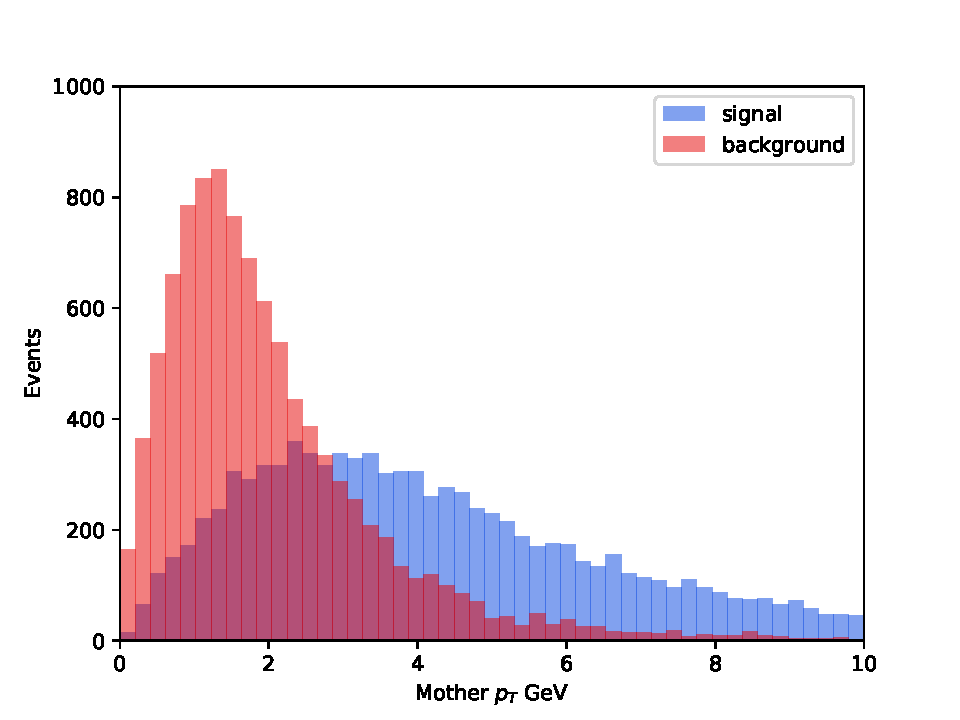
\includegraphics[width=0.33\textwidth]{pt_comp}
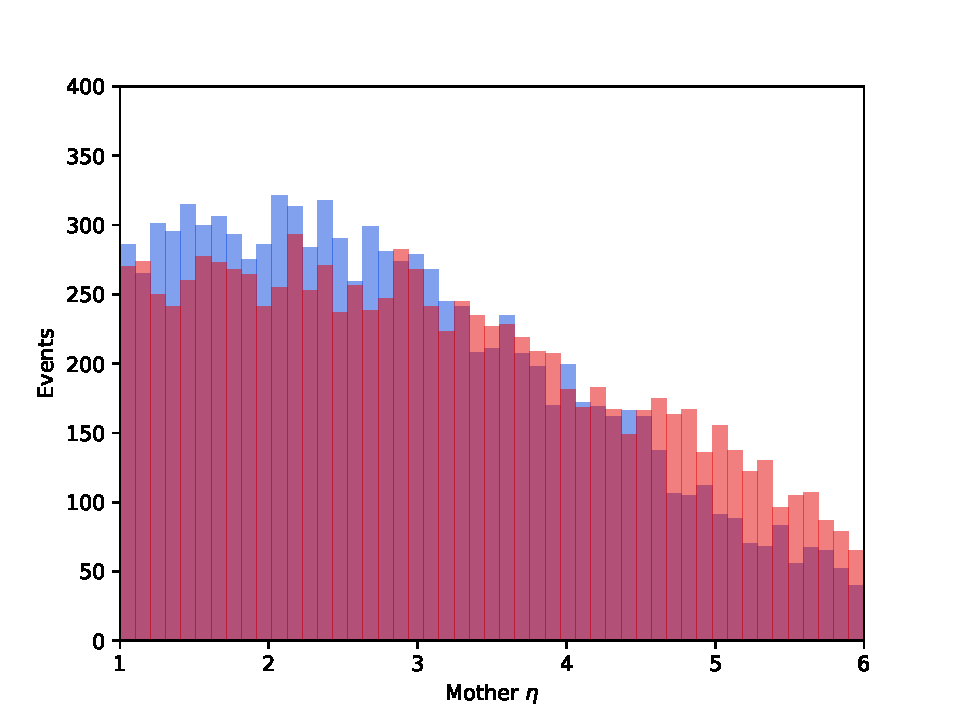
\includegraphics[width=0.33\textwidth]{eta_comp}
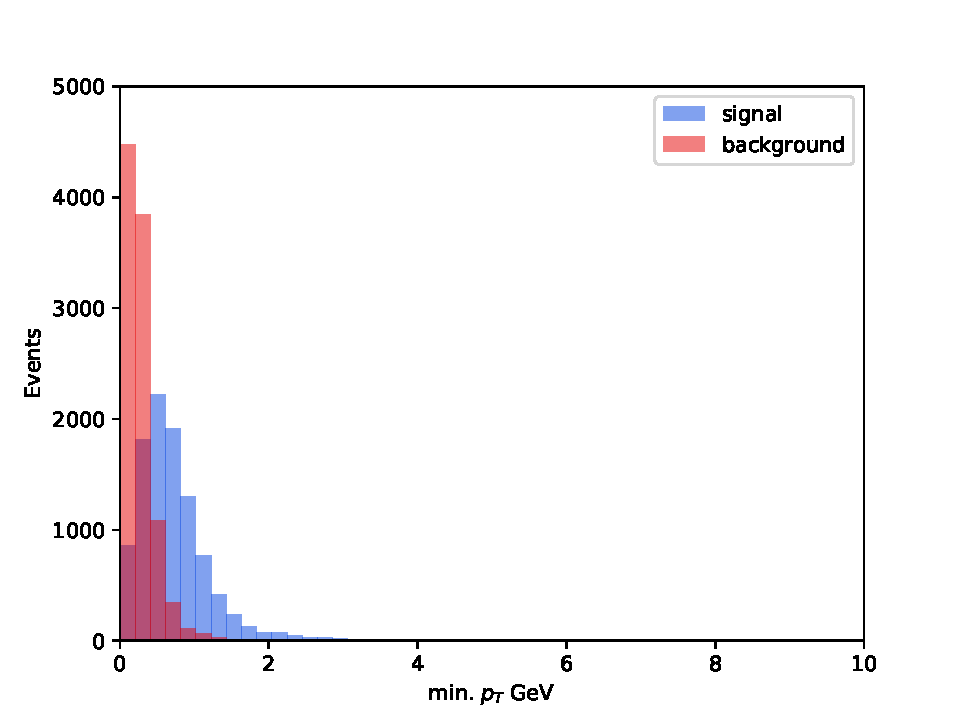
\includegraphics[width=0.33\textwidth]{minpt_comp}
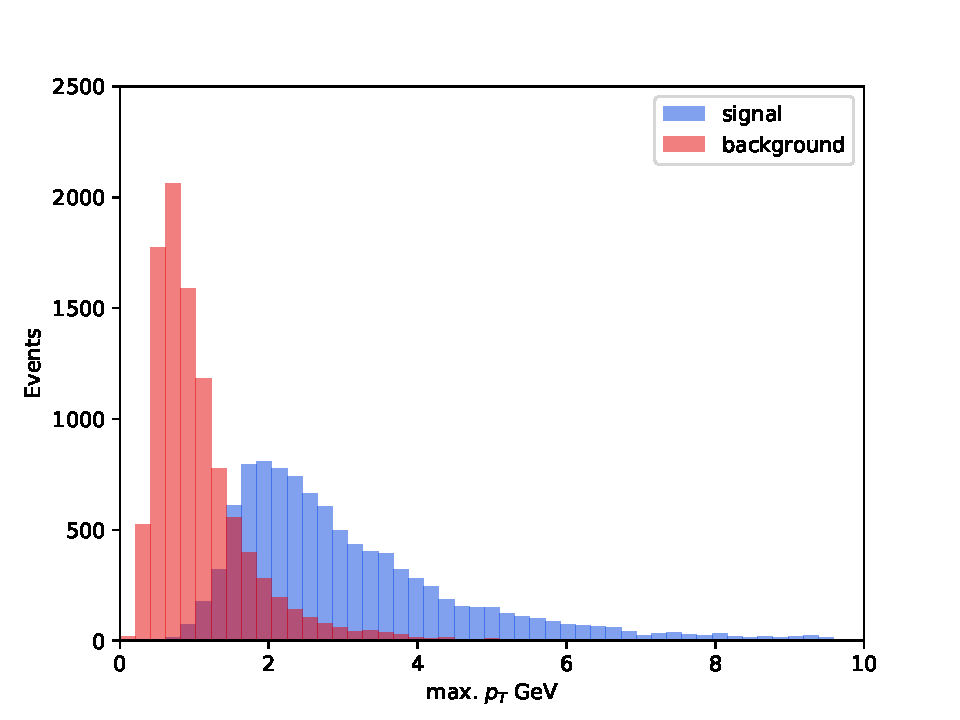
\includegraphics[width=0.33\textwidth]{maxpt_comp}
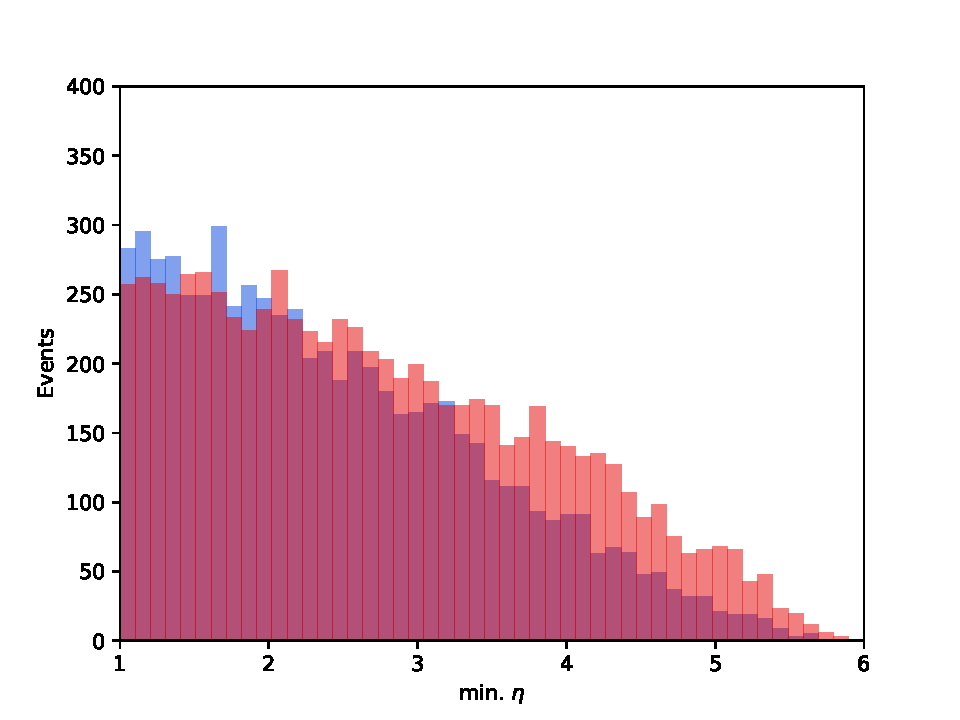
\includegraphics[width=0.33\textwidth]{mineta_comp}
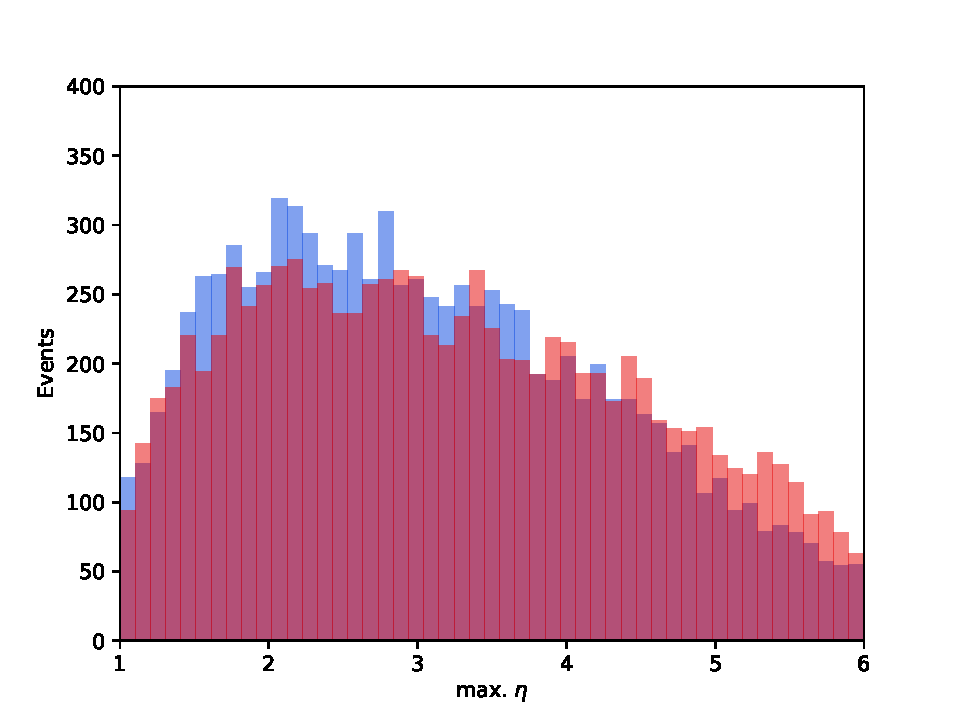
\includegraphics[width=0.33\textwidth]{maxeta_comp}
\caption{\small Comparison of the signal and background distributions
used to train the SciKit-Learn classifier .}
\label{fig:inputs}
\end{figure*}

In the training of the original classifier, half of the data is
reserved in order to test for overtraining.
%The output probability distributions of the signal and background samples
%after the training are shown in Fig.~\ref{fig:output}.
%It can be seen that the test and training samples are in good agreement,
%showing that the original SciKit-Learn classifier is not significantly overtrained.
%\begin{figure*}[t]
%\centering
%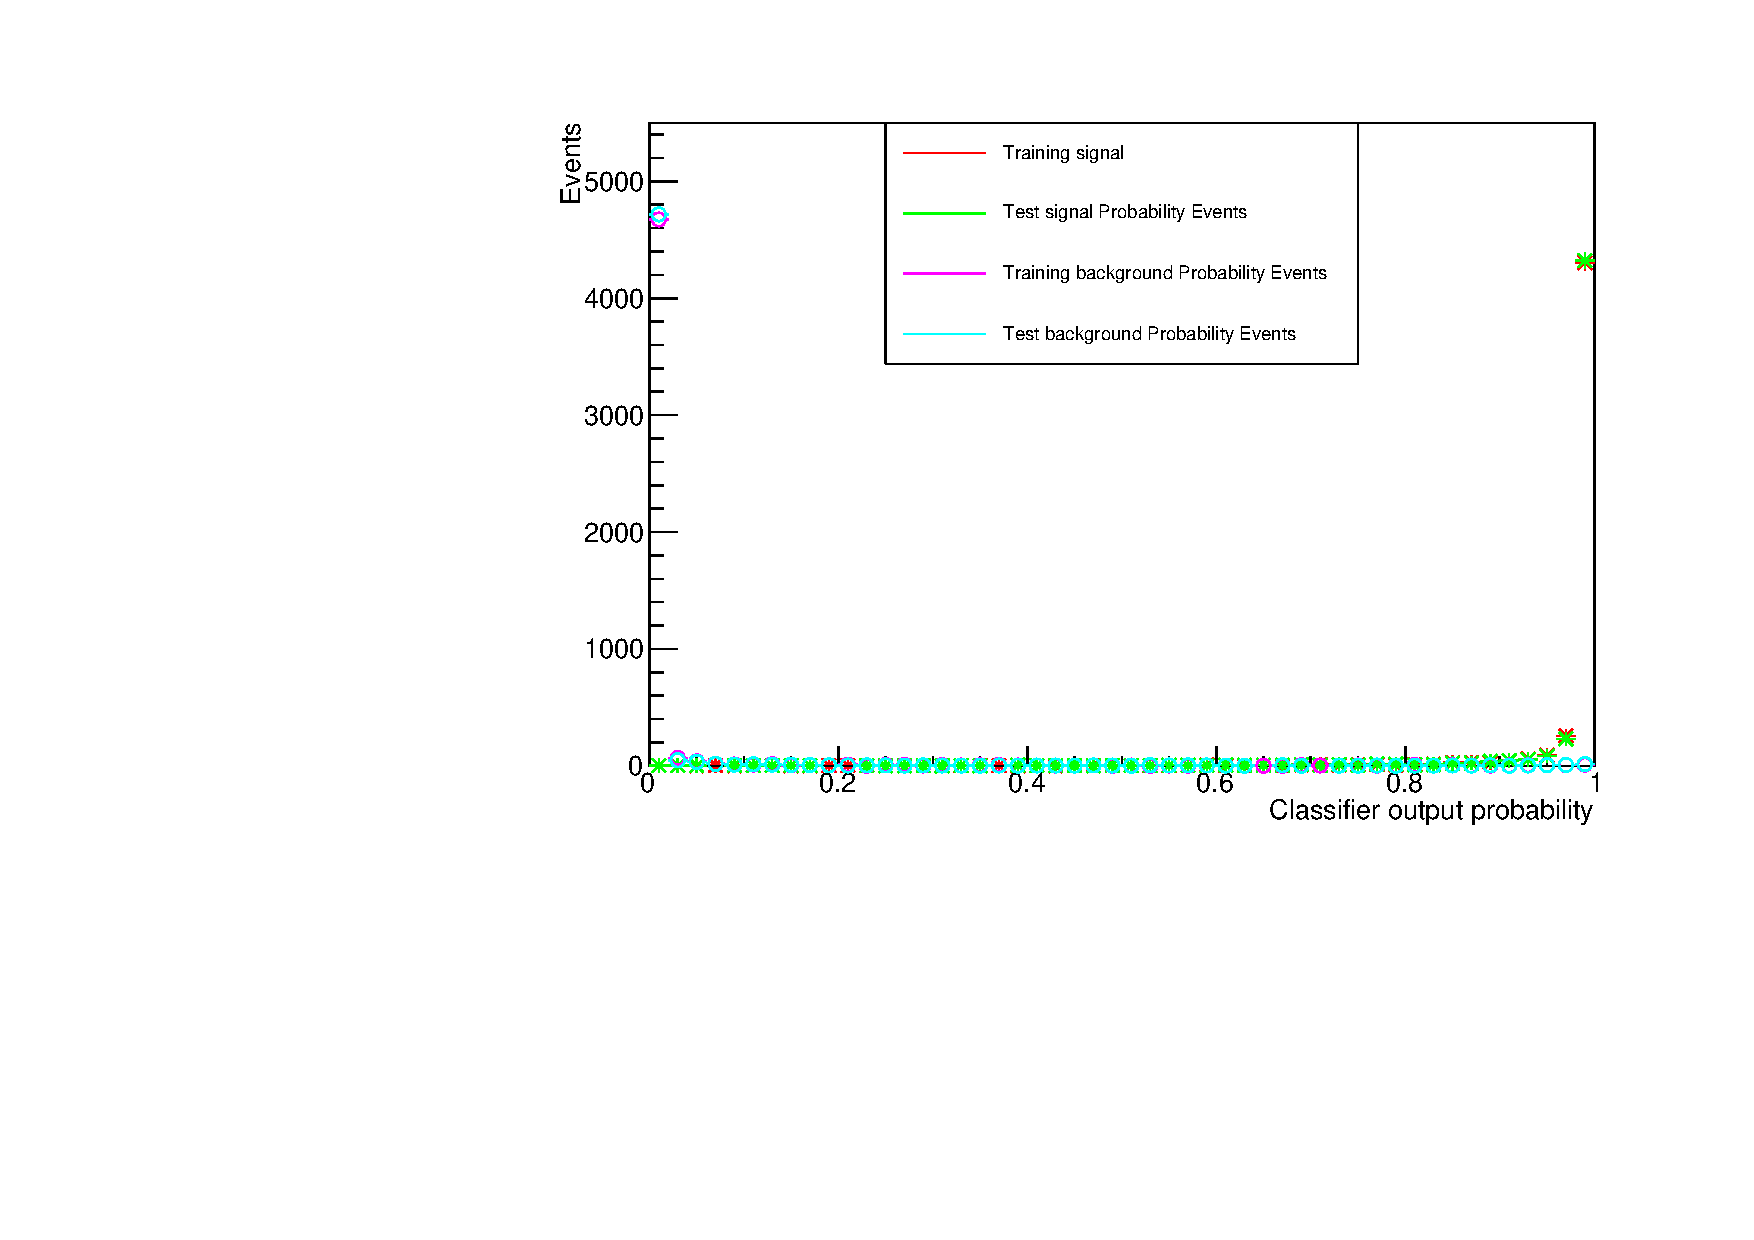
\includegraphics[width=0.45\textwidth]{event_probability}
%\caption{\small 
%Output distributions of the signal and background training and
%test samples from the classifier after training.
%}
%\label{fig:output}
%\end{figure*}

\subsection{Drone conversion}

The drone neural network is trained following the procedure outlined in Sec.~\ref{sec:dlearn},
In total, 300 epochs are used with
the learning rate of the stochastic gradient descent set to 0.05.
The value of $\kappa$ is chosen to be 0.02.

The loss history of the training is shown in Fig.~\ref{fig:loss}
as a function of epoch number.
The convergence is also shown in Fig.~\ref{fig:iterdiff}, which shows
the difference in the value of the loss function with respect to the previous
epoch. The epochs that triggered an increase in the number of hyperparameters
are also overlaid.
In total in this example, an increase was triggered 104 times. The total number
of parameters in the final drone neural network is therefore 3233. It is interesting
to note that with the algorithm design of Sec.~\ref{sec:dlearn}, the introduction
of the new parameter space causes the drone network to learn faster, as evidenced by
increases in Fig.~\ref{fig:iterdiff} with continuing descent of the loss function.
%
The performance of the original classifier and the drone classifier is shown in Figure~\ref{fig:roc}.
\begin{figure*}[t]
\centering
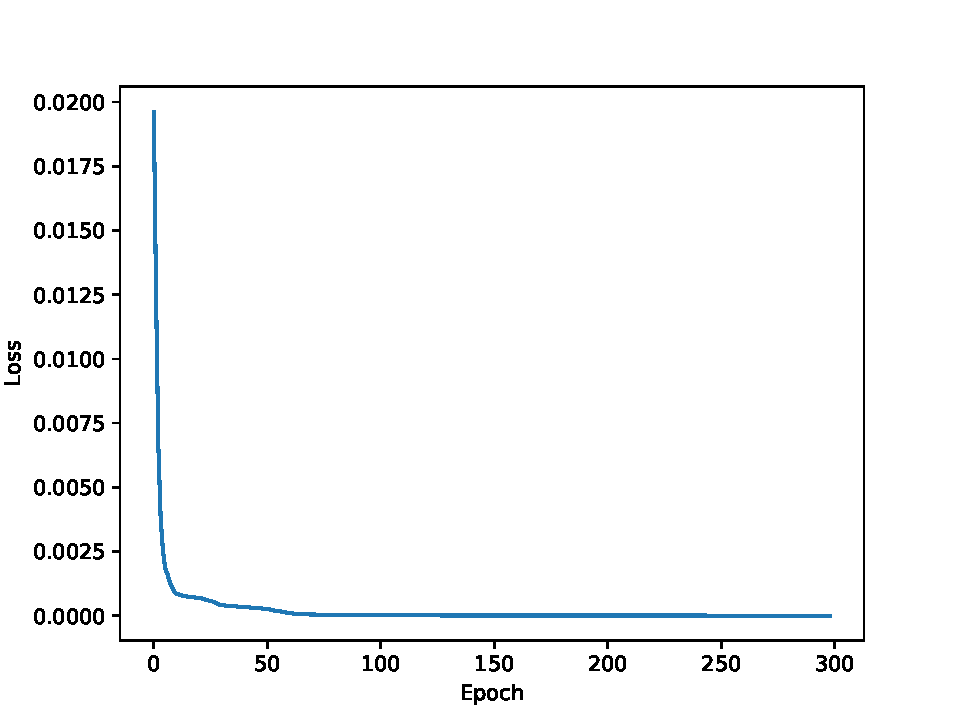
\includegraphics[width=0.45\textwidth]{loss_history}
\caption{\small 
Convergence of the loss function during the drone training.
}
\label{fig:loss}
\end{figure*}
\begin{figure*}[t]
\centering
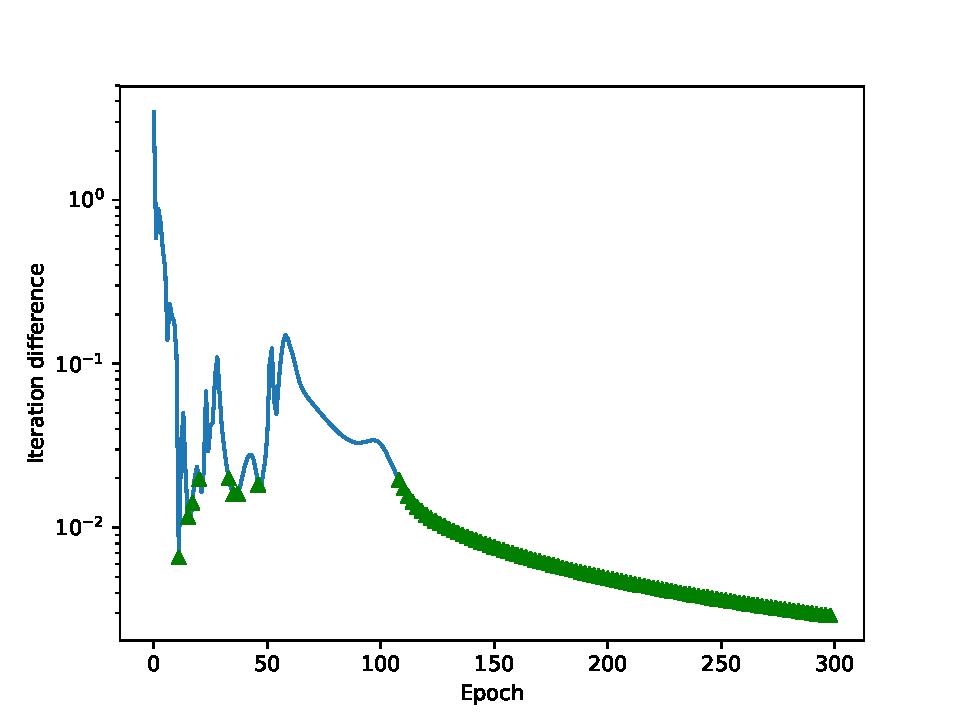
\includegraphics[width=0.45\textwidth]{diff_history}
\caption{\small 
Difference in the loss function with respect to the previous iteration. The green triangles
depict the epoch number in which the number of hyperperameters was increased.
}
\label{fig:iterdiff}
\end{figure*}
\begin{figure*}[t]
\centering
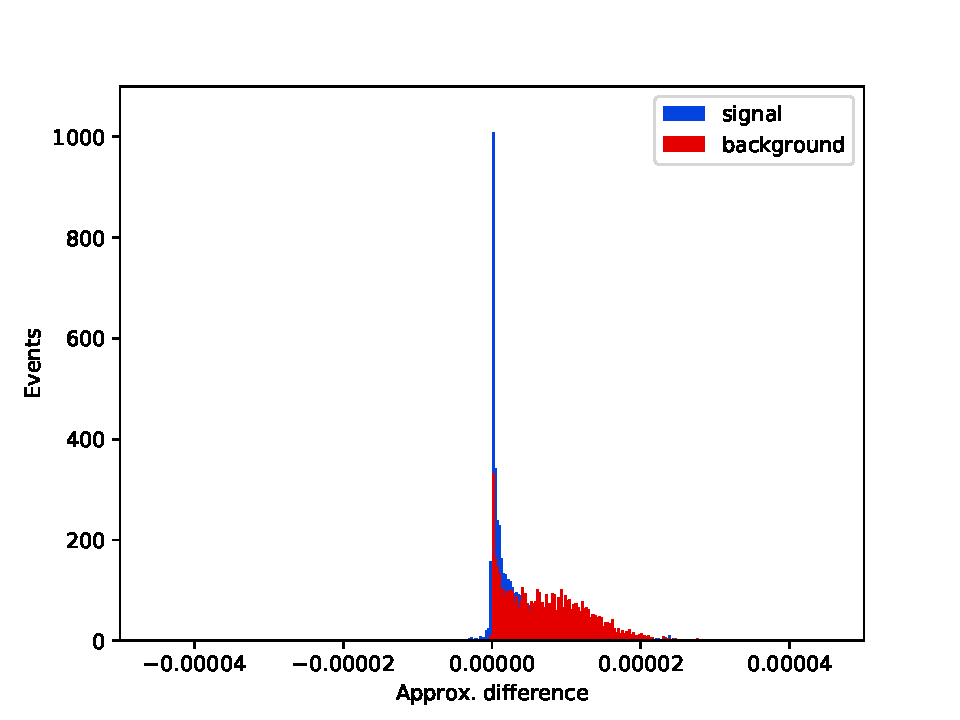
\includegraphics[width=0.45\textwidth]{approx_vs_truth_diff}
\caption{\small 
Difference between the output response of the drone model with respect to
the original classifier for data points in the test sample.
}
\label{fig:diff}
\end{figure*}


\section{High energy physics applications - Jet separation}
\label{sec:hepGPD}

\subsection{Data sample}

A further demonstration is provided demonstrating a classifiers ability to separate different
kinds of jets. The data sample to show this has been generated from Pythia~\cite{Sjostrand:2007gs}, using the FastJet~\cite{Cacciari:2011ma} package
to create the jet objects. 
The signal sample is chosen to be the jet produced in association with a W boson.
The background sample is chosen to be jets from Quantum Chromodynamics processes.

\subsection{Training of the original classifier}

The machine learning classifier chosen is a Keras-based convolutional neural net,
which is constructed as
\begin{lstlisting}
classifier = Sequential()
classifier.add(LocallyConnected1D(
filters = 90, kernel_size = 2, 
activation = 'sigmoid', 
input_shape = (len(setTrain[0]), 1)))
classifier.add(GlobalMaxPooling1D())
classifier.add(Dense(30, activation = 'sigmoid'))
classifier.add(Dense(1, activation = 'sigmoid'))
classifier.compile(optimizer = 'adam', 
loss = 'binary_crossentropy'
, metrics = ['accuracy'])
\end{lstlisting}

The neural network is trained using 4 jet properties consisting of the energy,
the combined mass of the particles in the jet, the pseudorapidity, and the jet $K_t$ (the definition 
of the $K_t$ variable and a review of jet reconstruction algorithms
may be found in Ref.~\cite{Atkin:2015msa}).
The signal and background distributions of the input variables
are shown in Fig.~\ref{fig:inputsGPD}.
%
\begin{figure*}[t]
\centering
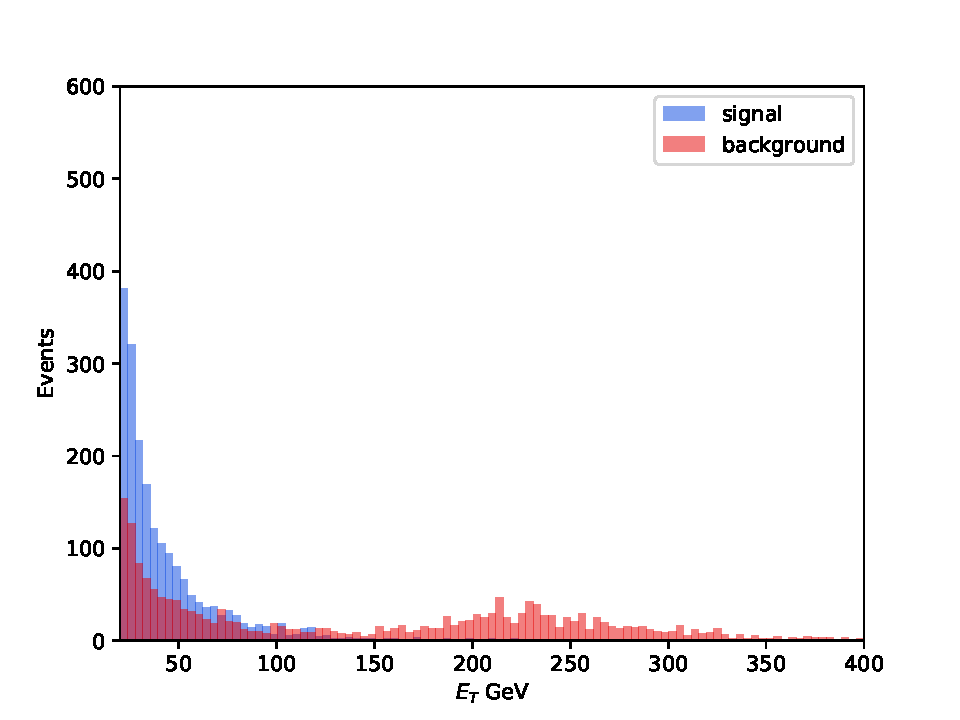
\includegraphics[width=0.33\textwidth]{et_comp_gpd}
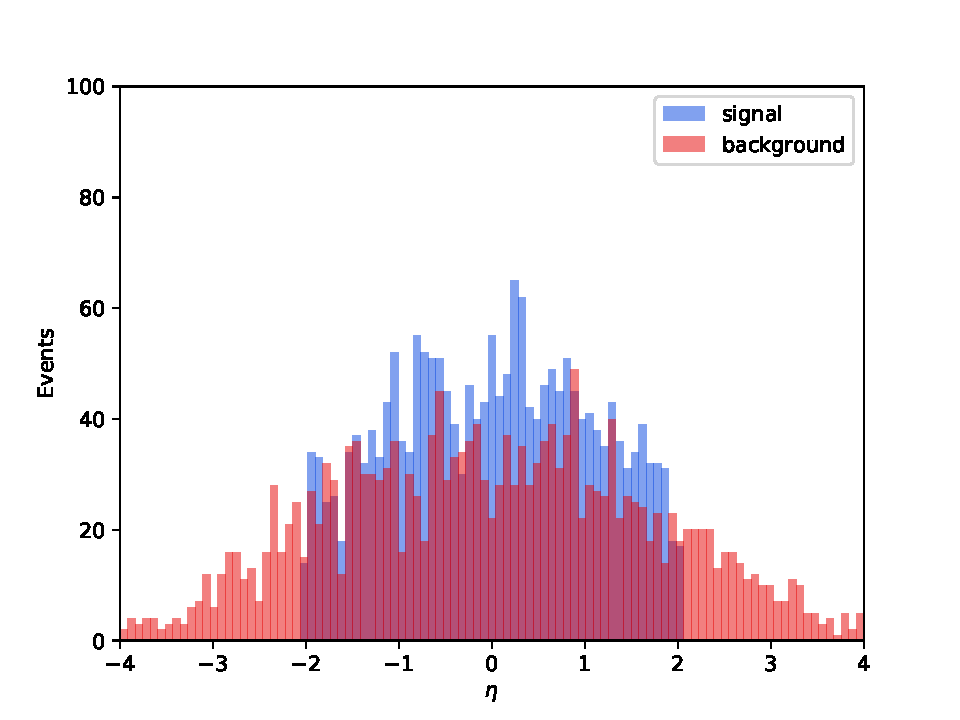
\includegraphics[width=0.33\textwidth]{eta_comp_gpd}
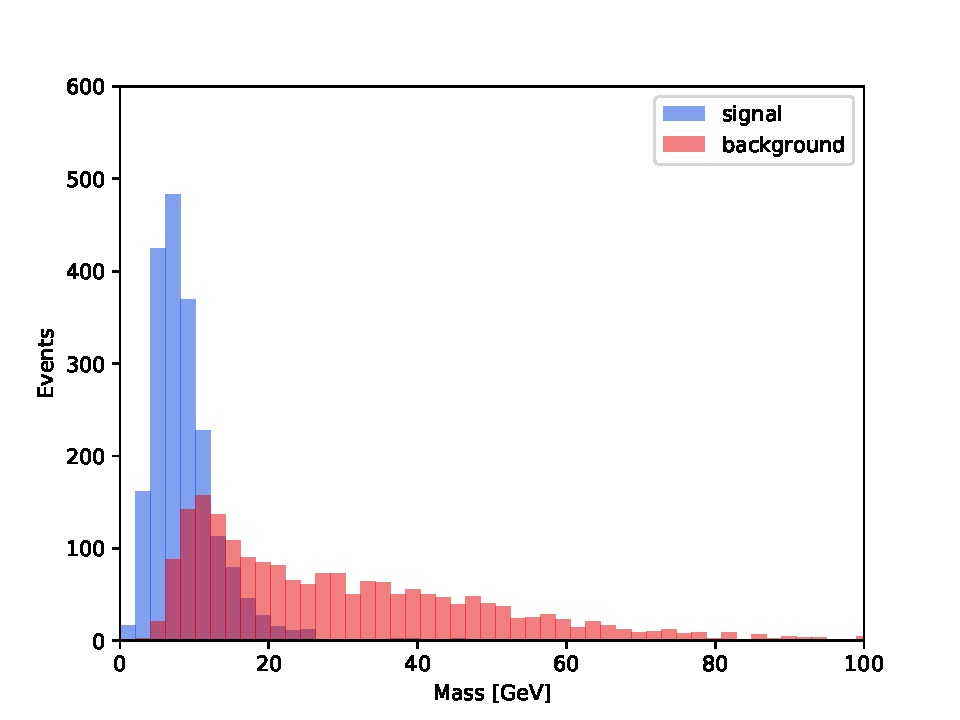
\includegraphics[width=0.33\textwidth]{m_comp_gpd}
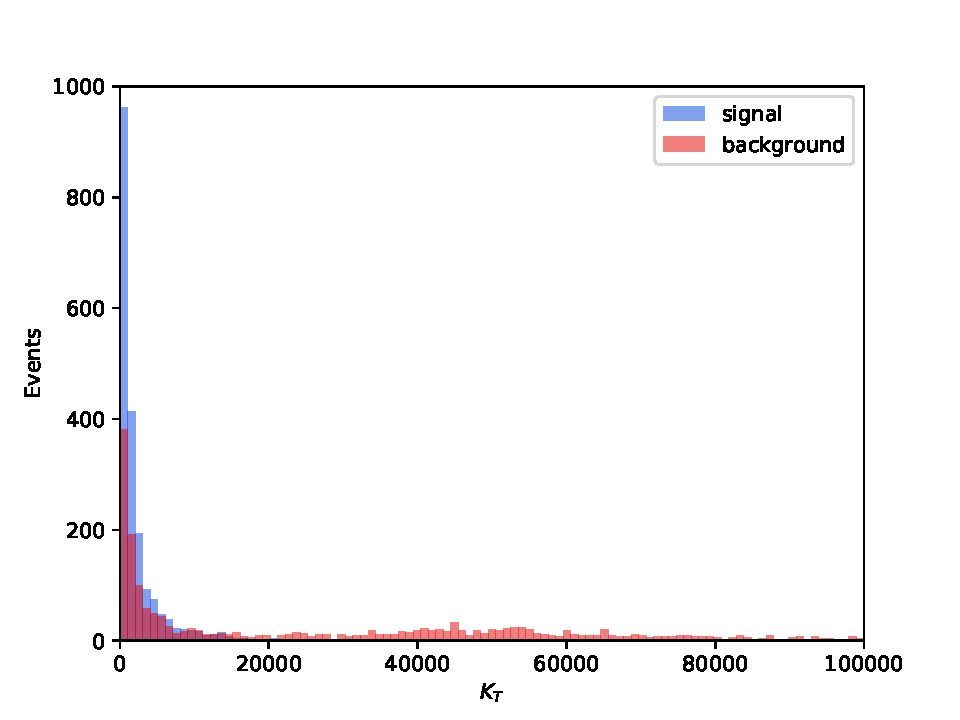
\includegraphics[width=0.33\textwidth]{kt_comp_gpd}
\caption{\small Comparison of the signal and background distributions
used to train the Keras classifier .}
\label{fig:inputsGPD}
\end{figure*}

\section{Drone storage and transferability}
\label{sec:storage}

The hyperparameters and structure of the drone are required to be 
portable and easily stored for later usage. For this the {\tt JSON} format was chosen as 
mediator. It is human-readable and easily accessible in the {\tt Python} and {\tt C++}
environments commonly used in HEP. Thus, it is readily deployable in both personal and production environments.

Provided is a tool to export and save a drone neural network to a {\tt JSON} 
formatted file which preserves the input \& output structure, 
the layers and nodes, all hyperparameters and activation functions. 
The drone configuration is later read in by an equivalent tool into the production software framework,
which then constructs a class object based on the Keras model. The {\tt C++} class implements 
a flexible member structure that is capable of completely reproducing the original drone. The production
implementation may be used for all data reduction levels, be it in the form of a low-latency trigger
for example up to the latest stages of data handling and output. 

A major advantage of this method is that analysts and users have the full freedom of latest developments
of industry standards, but need only to support a more manageable implementation in the low-latency
software.


\section{Summary}
\label{sec:summary}

It has been demonstrated that for the case of a high energy physics
event selection application, a drone neural network is able to accurately
approximate and learn the features of a neural network with a different
structure. The proposed algorithm design allows the drone to learn the
aforementioned features without ever having access to the training data,
or indeed any data, but only with appropriate questioning of the original model.

The equivalency of the outputs of the drone and original model enables an
analyst to treat both the original and the drone in the same way. The creation
of a drone in a standardised form permits an analyst to use any desired machine-learning
package to isolate a decay signature, and from this create a classifier
guaranteed to be suitable for execution in the {\tt C++} real-time data selection frameworks.


% Do not include this in analysis note and conference reports
\section*{Acknowledgements}

\noindent 
We acknowledge support from 
the NWO (The Netherlands) and STFC (United Kingdom).
We are indebted to the communities behind the multiple open 
source software packages on which we depend.
This project has received funding from the European Union’s Horizon 
2020 research and innovation programme under the Marie Skłodowska-Curie 
grant agreement No 676108.


% This should be taken out in the final paper
%\addcontentsline{toc}{section}{References}
\setboolean{inbibliography}{true}
\bibliographystyle{elsarticle-num}
\bibliography{main}
\begin{comment}
\begin{thebibliography}{10}
\expandafter\ifx\csname url\endcsname\relax
  \def\url#1{\texttt{#1}}\fi
\expandafter\ifx\csname urlprefix\endcsname\relax\def\urlprefix{URL }\fi
\expandafter\ifx\csname href\endcsname\relax
  \def\href#1#2{#2} \def\path#1{#1}\fi

\bibitem{Alves:2008zz}
A.~A. Alves~Jr., et~al., {The \lhcb detector at the LHC}, JINST 3 (2008)
  S08005.
\newblock \href {http://dx.doi.org/10.1088/1748-0221/3/08/S08005}
  {\path{doi:10.1088/1748-0221/3/08/S08005}}.

\bibitem{LHCb-DP-2014-002}
R.~Aaij, et~al., {LHCb detector performance}, Int. J. Mod. Phys. A30 (2015)
  1530022.
\newblock \href {http://arxiv.org/abs/1412.6352} {\path{arXiv:1412.6352}},
  \href {http://dx.doi.org/10.1142/S0217751X15300227}
  {\path{doi:10.1142/S0217751X15300227}}.

\bibitem{Xu:2016mik}
Z.~Xu, M.~Tobin, {Novel real-time alignment and calibration of the LHCb
  detector in Run II}, Nucl. Instrum. Meth. A824 (2016) 70--71.
\newblock \href {http://dx.doi.org/10.1016/j.nima.2015.11.040}
  {\path{doi:10.1016/j.nima.2015.11.040}}.

\bibitem{Aaij:2016rxn}
R.~Aaij, et~al., {Tesla : an application for real-time data analysis in High
  Energy Physics}, Comput. Phys. Commun. 208 (2016) 35--42.
\newblock \href {http://arxiv.org/abs/1604.05596} {\path{arXiv:1604.05596}},
  \href {http://dx.doi.org/10.1016/j.cpc.2016.07.022}
  {\path{doi:10.1016/j.cpc.2016.07.022}}.

\bibitem{Hocker:2007ht}
A.~Hocker, et~al., {TMVA - Toolkit for Multivariate Data Analysis}, PoS ACAT
  (2007) 040.
\newblock \href {http://arxiv.org/abs/physics/0703039}
  {\path{arXiv:physics/0703039}}.

\bibitem{Feindt:2006pm}
M.~Feindt, U.~Kerzel, {The NeuroBayes neural network package}, Nucl. Instrum.
  Meth. A559 (2006) 190--194.
\newblock \href {http://dx.doi.org/10.1016/j.nima.2005.11.166}
  {\path{doi:10.1016/j.nima.2005.11.166}}.

\bibitem{Pedregosa:2012toh}
F.~Pedregosa, et~al., {Scikit-learn: Machine Learning in Python}, J. Machine
  Learning Res. 12 (2011) 2825--2830.
\newblock \href {http://arxiv.org/abs/1201.0490} {\path{arXiv:1201.0490}}.

\bibitem{keras}
F.~Chollet, et~al., Keras, \url{https://github.com/fchollet/keras} (2015).

\bibitem{Barrand:2001ny}
G.~Barrand, et~al., {GAUDI - A software architecture and framework for building
  HEP data processing applications}, Comput. Phys. Commun. 140 (2001) 45--55.
\newblock \href {http://dx.doi.org/10.1016/S0010-4655(01)00254-5}
  {\path{doi:10.1016/S0010-4655(01)00254-5}}.

\bibitem{Gligorov:2012qt}
V.~V. Gligorov, M.~Williams, {Efficient, reliable and fast high-level
  triggering using a bonsai boosted decision tree}, JINST 8 (2013) P02013.
\newblock \href {http://arxiv.org/abs/1210.6861} {\path{arXiv:1210.6861}},
  \href {http://dx.doi.org/10.1088/1748-0221/8/02/P02013}
  {\path{doi:10.1088/1748-0221/8/02/P02013}}.

\bibitem{losssurfaces}
A.~Choromanska, M.~Henaff, M.~Mathieu, G.~B. Arous, Y.~LeCun,
  \href{http://arxiv.org/abs/1412.0233}{The loss surface of multilayer
  networks}, CoRR abs/1412.0233.
\newblock \href {http://arxiv.org/abs/1412.0233} {\path{arXiv:1412.0233}}.
\newline\urlprefix\url{http://arxiv.org/abs/1412.0233}

\bibitem{rapid}
G.~A. Cowan, D.~C. Craik, M.~D. Needham, {RapidSim: an application for the fast
  simulation of heavy-quark hadron decays}, Comput. Phys. Commun. 214 (2017)
  239--246.
\newblock \href {http://arxiv.org/abs/1612.07489} {\path{arXiv:1612.07489}},
  \href {http://dx.doi.org/10.1016/j.cpc.2017.01.029}
  {\path{doi:10.1016/j.cpc.2017.01.029}}.

\end{thebibliography}
\end{comment}

\end{document}
